
%*****************************************
\chapter{Materials and Methods}\label{ch:methods}
%*****************************************

\section{Aieouad\^o's dictionary and G2P converter}\label{sec:aieouado}
\footnote{This section contains is an extended version of the paper}
Aeiouad\^o is a product and an original contribution of this Master's research. It was developed by \citeauthor{Mendonca2014} \cite{Mendonca2014}, after noticing that no prior work applied machine learning algorithms to grapheme to phoneme conversion in \ac{BP}.

To the best of our knowledge, all previous efforts to solve the G2P problem in \ac{BP} used only a rule-based approach, and as such, they require complex linguistic knowledge to code rules and are difficult to evaluate. Unfortunately, it is a common practice in rule-based G2P (and a wrong one!) to develop the transcription rules based on a corpus and to evaluate them on the same corpus. This usally leads to overfitting, so that the results which are reported (some of them which approach 100\%) are hardly those which are found when such systems are applied to other data or tested in a different context. In addition to this, most of the G2P systems for \ac{BP} are proprietary or licensed under commercial terms, therefore their use is restricted.

We tried to overcome this gap by developing a hybrid G2P converter, which makes use of both rules and machine learning algorithms. The converter was evaluated with traditional machine learning metrics, such as precision, recall and F1-measure; therefore, its reported metrics are trustworthy. This converter was used to build a wide pronunciation dictionary, based on wordlist extracted from Wikipedia articles. Both the dictionary and the G2P converter are distributed under permissive licenses, respectivelly \ac{CC} and \ac{BSD}. Therefore, these resources aim at promoting the development of novel speech technologies for Brazilian Portuguese. It is interesting to notice that, despite being 6\textsuperscript{th} most spoken language in the world \cite{Ethnologue2013}, with about 200 million speakers, speech recognition and speech synthesis for Brazilian Portuguese are far from the current state of the art, specially what regard to open tools and resources \cite{Neto2011}. 

Aeiouad\^o's dictionary and G2P converter are based on the dialect of the city of S\~ao Paulo. They were designed primarily for Speech Technologies, such as \ac{ASR} an \ac{TTS}; but might also be used by linguists, speech therapists, lexicographers, students of Brazilian Portuguese as a second language, and whoever is interested in the sound structure of \ac{BP}.

The G2P converter makes use of a hybrid approach for grapheme to phoneme conversion, based on both manual transcription rules and machine learning algorithms. Hybrid approaches in grapheme to phoneme conversion have been applied successfully to other languages \cite{Damper1998, Polyakova2006, Teixeira2006, Veiga2013}. They have the benefit of taking advantage from both knowledge-based and data-driven methods. We proposed a method in which the phonetic transcription of a given word is obtained through a two-step procedure. Its primary word list derives from the Portuguese Wikipedia dump of 23\textsuperscript{rd} January 2014. We decided to use Wikipedia as the primary word list for the dictionary for many reasons: i) given its encyclopedia nature, it covers wide-ranging topics, providing words from both general knowledge and specialized jargon; ii) it contains around 168,8 million word tokens, being robust enough for the task; iii) it makes uses of crowdsourcing, lessening author's bias; iv) its articles are distributed through Creative Commons License. Wikipedia articles were transformed into plain text, tokenized and word types were extracted.

The dictionary makes use of a hybrid approach for grapheme to phoneme conversion, based on both manual transcription rules and machine learning algorithms, and aims at promoting the development of novel speech technologies for Brazilian Portuguese. Hybrid approaches in grapheme to phoneme conversion have been applied successfully to other languages \cite{Damper1998}\cite{Polyakova2006}\cite{Teixeira2006}\cite{Veiga2013}. They have the benefit of taking advantage from both knowledge-based and data-driven methods. We propose a method in which the phonetic transcription of a given word is obtained through a two-step procedure. Its primary word list derives from the Portuguese Wikipedia dump of 23\textsuperscript{rd} January 2014. We decided to use Wikipedia as the primary word list for the dictionary for many reasons: i) given its encyclopedia nature, it covers wide-ranging topics, providing words from both general knowledge and specialized jargon; ii) it contains around 168,8 million word tokens, being robust enough for the task; iii) it makes uses of crowdsourcing, lessening author's bias; iv) its articles are distributed through Creative Commons License. Wikipedia articles were transformed into plain text, tokenized and word types were extracted.

We developed a language identifier in order to detect loanwords among data. It is a known fact that when languages interact, linguistic exchanges inevitably occur. One particular type of linguistic exchange is of great concern while building a pronunciation dictionary, namely, non-assimilated loanwords \cite{Bussmann96}. Non-assimilated loanwords stand for lexical borrowings in which the borrowed word is incorporated from one language into another straightforwardly, without any translation or orthographic adaptation. These words represent a problem to grapheme-to-phoneme (G2P) conversion since they show orthographic patterns which are not predicted in advance by rules or which are too deviant to be captured by machine learning algorithms. Many algorithms have been proposed to address Language Identification (LID) from text \cite{Bergsma2012, Bilcu2006, Dolf2012, Zampieri2012}. Since our goal is to detect the language of single words, we employed n-gram character  models in the identifier, given its previous success in dealing with short sequences of characters. 

Brazilian Portuguese Phonology can be regarded as syllable and stress-driven \cite{Cristofaro2005}. In fact, many phonological processes in Brazilian Portuguese are related to or conditioned by syllable structure and stress position \cite{Girelli1990}. Vowel harmony occurs in pretonic context \cite{Bisol1989}, posttonic syllables show a limited vowel inventory \cite{Cristofaro2005}, nasalization occurs when stress syllables are followed by nasal consonants \cite{Quicoli1990}, epenthesis' processes are triggered by the occurrence of non-allowed consonants in coda position \cite{Delatorre2005} and so on and so forth. Therefore, detecting syllable boundaries and stress is of crucial importance for G2P systems, in order to achieve correct transcriptions. Several algorithms have been proposed to deal with the syllabification in Brazilian Portuguese. However most of them were not extensively evaluated nor were made publicly available \cite{Oliveira2005, Nhenhem2012, Neto2011, Rocha2013}. For this reason, we implemented our own syllabification algorithm, 
based directly on the rules of the last Portuguese Language Orthographic Agreement \cite{Acordo2009}. 

Word types recognized as belonging to Brazilian Portuguese by the language identifier were transcribed in a two-step process: i) words are submitted to a set of transcription rules, in which predictable graphemes (mostly consonants) are transcribed; ii) a machine learning classifier is used to predict the transcription of the remaining graphemes (mostly vowels). All the data were subsequently revised. Figure 1 summarizes the method.

\begin{figure}[t]
\centerline{ 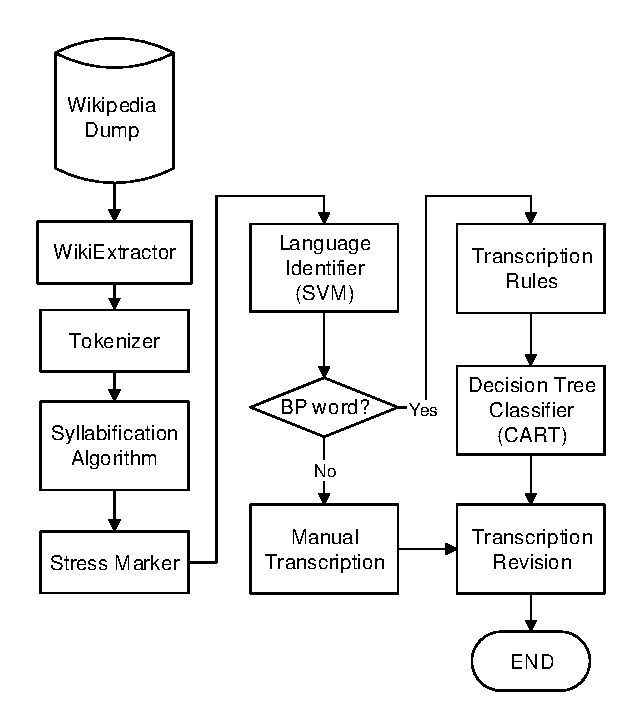
\includegraphics[width=8cm]{./gfx/flowchart_mod.pdf}}
\caption{{\it System architecture for building the pronunciation dictionary.}}
\label{g2p-architecture}
\end{figure}

We used the Portuguese Wikipedia's dump of 23\textsuperscript{rd} January 2014 as the primary word list for the pronunciation dictionary. In order to obtain plain text from the articles, we employed WikiExtractor \cite{Wikiextractor2013}; it strips all the  MediaWiki markups and metadata forms. Afterwards, texts were tokenized and unique words types extracted. The Portuguese Wikipedia has about 168,8 million word tokens and 9,7 million types, distributed among  820,000 articles. With the purpose of avoiding misspellings, URLs and other spurious data, only words with frequency higher than 10, which showed neither digits nor punctuation marks were selected. 

A Language Identifier module was developed in order to detect loanwords in the pronunciation dictionary. The Identifier consists of a Linear Support Vector Machine Classifier \cite{Steinwart2008} and was implemented in Python, through Scikit-learn \cite{Scikit2011}. It was trained on a corpus made of the 200,000, containing 100,000 Brazilian Portuguese words and 20,000 words of each of the following languages: English, French, German, Italian and Spanish. All of these words were collected through web crawling News' sites and were not revised. We selected these languages because they are the major donors of loanwords to Brazilian Portuguese \cite{Alves2001}. From these words we extracted features such as initial and final bi- and trigraphs;  number of accented graphs, vowel-consonant ratio; average mono-, bi- and trigraphs probability; and used them to estimate the classifier. Further details can be found in the website of the Project\footnote{http://nilc.icmc.usp.br/listener/aeiouado}. After training, we applied the classifier to the Wikipedia word list with the purpose of identifying loanwords among data. The identified loanwords were then separated from the rest of words for later revision, i.e. they were not submitted to automatic transcription.

Our syllabification algorithm follows a rule-approach and is based straightforwardly on the syllabification rules described in the Portuguese Language Orthographic Agreement \cite{Acordo2009}. Given space limitations, rules were omitted from this paper as they can be found in the website of the project, along with all the resources developed for the dictionary. As for the stress marker, once the syllable structure is known in Brazilian Portuguese, one can predict where stress falls. Stress falls:

\begin{enumerate}
 \item on the antepenultimate syllable if it has an accented vowel $<$\'a,\^a,\'e,\^e,\'i,\'o,\^o,\'u$>$;
 \item on the ultimate syllable if it contains the accented vowels $<$\'a,\'e,\'o$>$ or $<$i,u$>$; or if it ends with one of the following consonants $<$r,x,n,l,z$>$;
 \item on the penultimate syllable otherwise.
\end{enumerate}

The transcriber is based on a hybrid approach, making use of manual transcription rules and an automatic classifier, which builds Decision Trees. Initially, transcription rules are applied to the words. The rules covers not all possible graphemes to phoneme relations, but only those which are predictable by context. The output of the rules is what we called the intermediary transcription form. After obtaining it, a machine learning classifier is applied in order to predict the transcription of the remaining graphemes. Figure 2 gives an example of the transcription process.

\begin{figure}[!ht]
\centerline{ 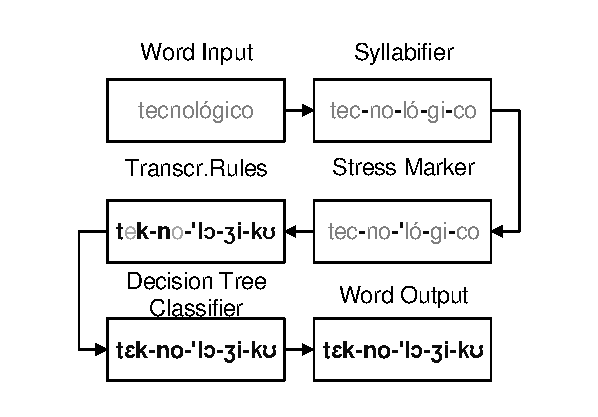
\includegraphics[width=8cm]{./gfx/transcript_ex.pdf}}
\caption{{\it Example of the transcription procedure -- in grey: graphemes yet to be transcribed; in black: graphemes already transcribed.}}
\label{transcExample}
\end{figure}

The rules' phase has two main goals: guarantee the correct transcription of certain predictable graphemes (mostly consonants) and also ensure the alignment between graphemes and phones for the classifier. They were set in order to avoid overlapping and order conflicts. Long sequences of graphemes, such as triphthongs, contextual diphthongs and general diphthongs are transcribed first (e.g.  $<$x-ce$> \rightarrow $\textipa{[-se]}). Then graphemes involving phones that undergo phonological processes are transcribed (e.g. $<$ti$> \rightarrow $\textipa{[tSi]}, $<$di$> \rightarrow $\textipa{[dZi]}). After that, several contextual and general monophones are transcribed (e.g. $<$\#x$> \rightarrow $\textipa{[S]}, $<$\#e-x$> \rightarrow $\textipa{[}\#\textipa{e-z]}). 

On what regards to the classifier, it was developed primarily to deal with the transcription of vowels. In Brazilian Portuguese, vowels have a very irregular behavior, specially the mid ones. Therefore the relations between the vowels' graphemes and their corresponding phonemes are hard to predict beforehand through rules. Consider, for instance, the words ``teto'' \emph{(roof)} and ``gueto'' \emph{(ghetto)}; both are nouns and share basically the same orthographic environment. However the former is pronounced with an open ``e'' \textipa{["tE.tU]} and the latter with a closed one \textipa{["ge.tU]}. The classifier employs Decision Trees, through an optimised version of the CART (Classification and Regression Trees) algorithm and was implemented in Python, by means of the Scikit-learn library \cite{Scikit2011}. 

The algorithm was trained over a corpus of 3,500 words phonetically transcribed and manually revised, with a total of 39,934 instances of phones. The feature extraction happened in the following way. After reviewing the data, we obtained the intermediary transcription form for each of these words and aligned them with the manual transcription. Then, we split the intermediary transcription form into its corresponding phones and, for each phone, we extracted the following information: 

\begin{enumerate}
 \item the phone itself; 
 \item 8 previous phones; 
 \item 8 following phones; 
 \item the distance between the phone and the tonic syllable; 
 \item word class -- parts of speech; 
 \item the manually transcribed phone. 
\end{enumerate}

We considered a window of 8 phones in order deal with vowel harmony phenomena. By establishing a window with such length, one  can assure that pretonic phones will be able to reach the transcription of the vowels in the stressed syllable. The classifier was applied to all 108,389 words categorized as BP words by the Language Identifier module, all of them were cross-checked by two linguists with experience in Phonetics and Phonology.

The Portuguese Wikipedia has about 168,8 million word tokens and 9,7 million types, distributed among 820k articles. After applying the filters to the data, i.e. words with frequency higher than 10, with no digits nor punctuation marks, we ended up with circa 238k word types, representing 151,9 million tokens. Table 1 describes the data.

\begin{table} [t,h]
\caption{\label{wikipedia} {\it Portuguese Wikipedia Summary -- Dumped on 23\textsuperscript{rd} January 2014.}}
\vspace{2mm}
\centerline{
\begin{tabular}{ccc}
\hline \bf & \bf Word Tokens  & \bf Word Types\\\hline
Wikipedia & 168,823,100 & 9,688,039 \\
Selected  & 151,911,350 & 238,012 \\
\textbf{\% Used} &90.0 & 2.4 \\
\hline
\end{tabular}}
\end{table}

The selected words covers 90,0\% of the Wikipedia content. Although the number of selected word types seems too small at first glance, one of the reasons is that 7,901,277 of the discarded words were numbers (81,5\%). The remaining discarded words contained misspellings (\emph{dirijem-se} -- it should be \emph{dirigem-se}), used a non-Roman alphabet ($\lambda$\emph{\'o}$\gamma \omega$), were proper names (\emph{Stolichno}, \emph{Z\'e-pereira}), scientific names (\emph{Aegyptophitecus}), abbreviations or acronyms (LCD, HDMI). 

As for the language identifier, we trained and evaluated it with the 200,000 words multilingual corpus. The corpus consists of 100,000 Brazilian Portuguese words and 20,000 words from each of the following languages: English, French, German, Italian and Spanish. All of these words were collected through web crawling News' sites and were not revised. The results obtained for the identifier, through 5-fold cross validation are described in Table 2. 

\begin{table} [t,h]
\caption{\label{langIdentEval} {\it Results from the Language Identifier module -- Training Phase.}}
\vspace{2mm}
\centerline{
\begin{tabular}{ccccc}
\hline
 & \textbf{Precision} & \textbf{Recall} & \textbf{F1-score} & \textbf{Support} \\ \hline
BP words & 0.85 & 0.89 & 0.87 & 100,000 \\ 
Foreign Words & 0.88 & 0.84 & 0.86 & 100,000 \\
\bf Avg/Total & 0.86 & 0.86 & 0.86 & 200,000 \\ \hline
\end{tabular}}
\end{table}

The language identifier showed an average F1-score of 0.86. Although such result is not as good as we expected -- some authors reported 99\% by using similar methods with trigrams probability, the relatively low F1-score can be explained given the nature of the data. In most language identifiers, the input  consists of texts or several sentences, in other words, there is much more data available for the classifier. Since we are working with single words, the confusion of the model is higher and the results are, consequently, worse. Additionally, because the word list used to train the identifier was not revised, there is noise among the data. After training and evaluating the classifier, we applied it to the selected word list derived from the Wikipedia, in order to detect loanwords. Table 3 describes the results gathered.

\begin{table} [H]
\caption{\label{langIdentWiki} {\it Results from the Language Identifier module -- Wikipedia word list.}}
\vspace{2mm}
\centerline{
\begin{tabular}{cc}
\hline
 & \textbf{Wikipedia word list}\\ \hline
BP words & 108,370 (46\%)\\ 
Foreign Words & 129,642 (54\%)\\
\bf Total & 238,012 \\ \hline
\end{tabular}}
\end{table}

As one can observe, although we established a frequency filter to avoid spurious words, many loanwords still remain. More than half of the word list selected from Wikipedia consists of foreign words. Notwithstanding that, the list of Brazilian Portuguese words is still of considerable size. For instance, the CMUdict \cite{CMUdict1998}, a reference pronunciation dictionary for the English language, has about 125,000 word types.

Concerning the syllabification algorithm and the stress marker, we did not evaluate them in isolation, but together with the transcriber since the rules for each of these modules are intertwined. That is to say the transcription rules are strictly dependent on the stress marker module and the syllable identifier. Besides, the Decision Tree Classifier is built upon the output of the transcription rules, so it is entirely dependent on it. The Decision Tree Classifier was trained over a corpus of 3,500 cross-checked transcribed words, containing 39,934 instances of phones. We analyzed its performance through 5-fold cross validation, the results for each individual phone are summarized in Table 4.

\begin{table} [H]
\caption{\label{transcriberEval} {\it Results from the Transcriber -- Performance per phone.}}
\vspace{2mm}
\centerline{
\begin{tabular}{ccccc}
\hline
 & \bf Precision & \bf Recall & \bf F1-score & \bf Support \\ \hline
\emph{syl. boundary} & 1.00 & 1.00 & 1.00 & 9099 \\ 
\emph{stress} & 1.00 & 1.00 & 1.00 & 3507 \\ 
\textipa{p} & 1.00 & 1.00 & 1.00 & 760 \\ 
\textipa{b} & 1.00 & 1.00 & 1.00 & 357 \\ 
\textipa{t} & 0.99 & 0.99 & 0.99 & 1135 \\ 
\textipa{d} & 0.99 & 0.99 & 0.99 & 1148 \\ 
\textipa{k} & 0.99 & 0.99 & 0.99 & 978 \\ 
\textipa{g} & 1.00 & 1.00 & 1.00 & 298 \\ 
\textipa{tS} & 0.98 & 0.98 & 0.97 & 450 \\ 
\textipa{dZ} & 0.96 & 0.96 & 0.96 & 243 \\ 
\textipa{m} & 1.00 & 1.00 & 1.00 & 668 \\ 
\textipa{n} & 1.00 & 1.00 & 1.00 & 556 \\ 
\textipa{\textltailn} & 1.00 & 1.00 & 1.00 & 69 \\ 
\textipa{f} & 1.00 & 1.00 & 1.00 & 311 \\ 
\textipa{v} & 1.00 & 1.00 & 1.00 & 531 \\ 
\textipa{s} & 0.98 & 0.98 & 0.98 & 2309 \\ 
\textipa{z} & 0.93 & 0.94 & 0.93 & 416 \\ 
\textipa{S} & 0.84 & 0.84 & 0.84 & 138 \\ 
\textipa{k.s} & 0.72 & 0.64 & 0.66 & 41 \\ 
\textipa{Z} & 1.00 & 1.00 & 1.00 & 196 \\ 
\textipa{l} & 1.00 & 1.00 & 1.00 & 682 \\ 
\textipa{L} & 1.00 & 1.00 & 1.00 & 58 \\ 
\textipa{R} & 1.00 & 1.00 & 1.00 & 1388 \\ 
\textipa{h} & 0.98 & 0.99 & 0.99 & 737 \\ 
\textipa{H} & 0.97 & 0.92 & 0.94 & 169 \\ 
\textipa{w} & 0.97 & 0.98 & 0.97 & 441 \\ 
\textipa{\~w} & 0.98 & 0.99 & 0.99 & 309 \\ 
\textipa{j} & 0.97 & 0.95 & 0.96 & 223 \\ 
\textipa{\~j} & 0.95 & 1.00 & 0.98 & 110 \\ 
\textipa{a} & 1.00 & 1.00 & 0.99 & 2316 \\ 
\textipa{@} & 0.99 & 0.99 & 0.99 & 1093 \\ 
\textipa{E} & 0.65 & 0.68 & 0.66 & 275 \\ 
\textipa{e} & 0.93 & 0.91 & 0.92 & 1779 \\ 
\textipa{i} & 0.98 & 0.99 & 0.98 & 2073 \\ 
\textipa{I} & 0.97 & 0.97 & 0.97 & 365 \\ 
\textipa{O} & 0.69 & 0.75 & 0.71 & 220 \\ 
\textipa{o} & 0.93 & 0.92 & 0.93 & 1112 \\ 
\textipa{u} & 0.96 & 0.96 & 0.96 & 488 \\ 
\textipa{U} & 1.00 & 1.00 & 1.00 & 1033 \\ 
\textipa{\~a} & 1.00 & 1.00 & 1.00 & 719 \\ 
\textipa{\~e} & 0.96 & 0.97 & 0.97 & 497 \\ 
\textipa{\~i} & 0.99 & 0.99 & 0.99 & 274 \\ 
\textipa{\~o} & 0.97 & 0.96 & 0.97 & 299 \\ 
\textipa{\~u} & 0.94 & 0.92 & 0.93 & 64 \\ 
Avg/Total & 0.98 & 0.98 & 0.98 & 39934 \\ \hline
\end{tabular}}
\end{table}

As it can be seen, the method achieved very good results, with a F1-score of 0.98. Many segments were transcribed with 100\% accuracy, most of them were consonants. As it was expected, the worst results are related to mid vowels \textipa{[E, e, O, o]}, specially mid-low vowels, \textipa{[E]} showed a F1-score 0.66 and \textipa{[O]} of 0.71. It can be the case that since the grapheme context is the same for \textipa{[E, e]} and \textipa{[O, o]}, the DecisionTree classifier generalizes, in some cases, to the most frequent phone, that is the mid-high vowels \textipa{[e,o]}. The transcriber also had problems with the \textipa{[k.s]} (F1-score: 0.66) and \textipa{[S]} (F1-score: 0.84). This result was also expected, both these phones are related to the grapheme $<$x$>$ which, in Brazilian Portuguese, shows a very irregular behavior. In fact, $<$x$>$ can be pronounced as \textipa{[S, s, z, k.s]}, depending on the  word:  ``bruxa'' \emph{(witch)} \textipa{[S]}, ``pr\'oximo'' \emph{(near)} \textipa{[s]};  ``exame'' \emph{(test)} \textipa{[z]} and ``axila'' \emph{(armpit)} \textipa{[k.s]}.

We presented the method we employed in building a pronunciation dictionary for Brazilian Portuguese. High F1-score values were achieved while transcribing most of the graphemes in Brazilian Portuguese and the dictionary can be considered robust enough for Large Vocabulary Continuous Speech Recognition (LVCSR) and Speech Synthesis. Although the rules we developed are language-specific, the architecture we used for compiling the dictionary, by using transcription rules and machine learning classifiers, can be successfully replicated in other languages. In addition, the entire dictionary, all scripts, algorithms and corpora were made publicly available.\footnote{\url{http://nilc.icmc.usp.br/aeiouado}}\footnote{\url{https://github.com/gustavoauma/aeiouado_g2p}}

\clearpage

\paragraph{Further developments}

Since the publishing date of our paper (\citeauthor{Mendonca2014}~\cite{Mendonca2014}), Aeiouad\^o \ac{G2P} has been improved. Recently, we increased the training database to XXX words (XXX phone tokens). Moreover we are now using extra morphological information in order to determine the grapheme's transcription, mostly to solve the problems with the mid vowels \textipa{[E, e, O, o]}. 

Previously we were using only the parts of speech as the source of morphological information. We assumed that by just providing the words' parts of speech, the Decision Tree Classifier would be able to learn and differ pairs of heterophonic homographs, such as ``jogo'' \textsc{noun} \emph{(game)} and ``jogo'' \textsc{verb} \emph{(I play)}, or ``governo'' \textsc{noun} \emph{(government)} and ``governo'' \textsc{verb} \emph{(I rule)}. However, given the poor performance of the conversor in discerning between \textipa{[E]} vs. \textipa{[e]}, and \textipa{[O]} vs. \textipa{[o]}; we decided to refine the morphological features. 

We adapted the training database to the Unitex-PB dictionary \cite{Muniz2004}, which follows  formalismo DELA (Dictionnarie Electronique du LADL)

There is a huge lexicon with,

This type of alternation is very productive in \ac{BP}.  reported to have collected 1,812 pairs of heterophonic homographs in dictionaries and , although only 226 occurred in corpus).

\citeauthor{}, Pandu , although in a corpus analysis, only 226 \cite{Shulby2013}.

However this is not the case. Previously, only the word class information was used to determine. We thought that would be enough to 

\section{A Method for the Extraction of Phonetically-Rich Sentences}


\subsection{abstract}
A method is proposed for compiling a corpus of phonetically-rich triphone sentences; 
i.e., sentences with a high variety of triphones, distributed in a uniform fashion. 
Such a corpus is of interest for a wide range of contexts, from automatic speech 
recognition to speech therapy. We evaluated this method by building phonetically-rich corpora for Brazilian Portuguese. The data employed comes 
from Wikipedia's dumps, which were converted into plain text, segmentized and 
phonetically transcribed. The method consists of comparing the distance between 
the triphone distribution of the available sentences to an ideal uniform distribution, with 
equiprobable triphones. A greedy algorithm was implemented to recognize and evaluate 
the distance among sentences. A heuristic metric is proposed for pre-selecting 
sentences for the algorithm, in order to quicken its execution. The results show 
that, by applying the proposed metric, one can build corpora with more uniform 
triphone distributions.


\subsection{Introduction}

In what regards to speech technology, although there are some studies which employ words~\cite{Thanga2008}, syllables~\cite{Gana2001} and monophones~\cite{Kumar2014} to develop Automatic Speech Recognition (ASR) and Text to Speech (TTS) systems, most of the current research widely makes use of contextual phone units, such as triphones and diphones.

The issue of developing a phonetically-rich triphone sentences corpus is of great significance for many areas 
of knowledge. In many applications of  ASR and Speech Synthesis, for instance, rich speech databases are important for properly estimating the acoustic models \cite{Rabiner2007}. In Speech Therapy, phonetically-rich sentences are often employed in reading aloud tasks so as to assess the speech production of patients in various phonetic/phonological contexts \cite{Mendes2012}. Laboratory Phonologists
are also interested in such corpora in order to develop prompts for analyzing speech production and variability \cite{Pierrehumbert2000}.

Formally, the task discussed in this work can be described as follows: given a corpus $K$ with $s$ sentences,
find a subset $P$ containing $s_p$ sentences, such that the triphones that compose $s_p$ holds a 
uniform distribution as much as possible. Despite it's apparent simplicity, in what concerns computational complexity,
the task cannot be considered a simple one. Since it has a combinatorial nature, it lacks a polynomial-time
solution and should be regarded as an intractable problem \cite{Sedgewick2013}.

We evaluate the proposed method 
%for the extraction of sentences in order to
in building a phonetically-rich triphone sentences corpus for Brazilian Portuguese. The sentences come from the Portuguese Wikipedia dump 
\cite{Wikidump2014}, which was converted into plain text, segmentized and phonetically transcribed. The algorithm employs 
a greedy approach to select sentences, in a way such that the triphone distribution in the selected sentences is as uniform as possible. In order to expedite its execution, a heuristic metric is proposed 
to pre-select sentences for the algorithm, favoring the least frequent triphones over the most frequent ones.

The remainder of this paper is organized as follows. In Section 2, we briefly describe the related work available in the literature.In Section 3, we describe the method proposed. In Section 4, we evaluate it by building phonetically-rich corpora for Brazilian Portuguese. The final remarks are outlined in Section 5.


\subsection{Related Work}

Speech can be analyzed in a myriad of forms. The Phonetic or Phonological structure of a 
language can be described through phones, phonemes, syllables, diphones, triphones, feet, etc. 
For languages such as Mandarim, in which tones have a phonological value, one must even posit 
units such as tonemes in order to properly describe speech phenomena \cite{Lei2005}.

Many methods have been proposed for extracting phonetically-balanced corpora, that is to say 
corpora made of sentences which reproduce the triphone distribution of a given language 
\cite{Abushariah2012}\cite{Shen1994}\cite{Timit1993}\cite{Uraga2004}. 

It is known that many linguistic phenomena, including triphone sets, show a Zipfian distribution
 \cite{Manning1999}.
A phonetically-balanced corpus, for this reason, is a corpus which follows Zipf's law in 
representing each triphone inversely proportional to its rank in the frequency table. 

These kinds of corpora are important specially for Large Vocabulary Continuous Speech 
Recognition (LVCSR), where unbalanced triphone representations can achieve better Word Error 
Rates (WER). However, phonetically-balanced corpora are not adequate for many other tasks, 
even regarding Speech Recognition. When building a system  to assess one's pronunciation 
quality or to synthesize speech, for instance, more accurate results can be attained by 
using uniform triphone representations, i.e. phonetically-rich corpora. 

Phonetically-rich corpora in our work are those which show sentences with a high variety of 
triphones, distributed in a uniform fashion regardless its representation in the language. 
In other words, in order to build such corpora, Zipf's law must be nullified, by favoring 
less frequent triphones and disfavoring more frequent ones. However, there are studies that 
consider other definitions and even other basic units to build phonetically-rich corpora.

In Abushariah et al. \cite{Abushariah2012}, the concept of ``rich'' is used in the sense that the set must 
contain all the phonemes of Arabic language (the chosen language for their study) 
but without a need for a uniform distribution. The set of sentences was handmade 
developed by linguists/experts.They used a set of 663 words, also defined  by hand, 
and then Arabic independent sentences have been written using the 663 phonetically 
rich words. The final database consists of 367 sentences with 2 to 9 words per sentence.

Arora et al.\cite{Arora2004} considered syllables as the basic unit to extract automatically 
phonetically-rich sentences from a large text corpus of Indian language, 
justifying their choice because a syllable is the smallest segment of uterance. 
In their process to extract the sentences for a given corpus the chosen set 
should have the same distribution of syllabic words and also the same distribution 
of consonant, vowel and other symbols.

Nicodem et al.\cite{Nicodem2007} deals specifically with Brazilian Portuguese (BP) 
and proposed a method based on genetic algorithms to select a set of sentences 
for a speech syntesis system. Their goal was to select a recording corpus that would 
improve the phonetic and prosodic variability of the system. They tried to fulfill the 
gap of phonetically-balanced corpora available for BP does not consider prosody, that is, 
the available corpora only deals with phonetic representativeness without considering 
prosody representativeness.

They have worked with CETENFolha corpus (www.linguateca.pt/cetenfolha/) which has circa of 
1,5 million sentences in order to gather 4,000 sentences phonetically and prosodically 
rich, being 1,000 declatives, 1,000 partial interrogatives, 1,000 total interrogatives, 
500 alternatives and 500 exclamatives.   

Their approach is composed of 4 stages, including grapheme-to-phoneme conversion, 
prosodic annotation, feature vector representation, and selection. 
The authors obtain prosodic features based on the pitch (they use a TTS to obtain the pitch contour), identifying tone events (H+, H-, H, L, and L-, where H and L stands for high and low, respectively) and using N for neutral, 
for each syllabe. Using these features to represent each sentence, the execute a genetic algorithm to select a subset. Their paper, however, is not 
clear about how the fitness function meets both constraints (phonetic and prosodic) since 
their method only includes prosodic features.

\subsubsection{Heuristic Metric}

For the expedition of the sentence extraction through the greedy algorithm, due to its high time complexity order,
we set a heuristic metric to pre-select sentences and rank them according to the triphones they contained. The metric 
uses the probability of the triphones in  the Corpus in order to favor the least frequent triphones over the most frequent ones. 
It consists of a summation of the reciprocal probability for each triphone in the sentence.

Formally, this can be defined in the following way. Consider a corpus $K$ consisting of a set of sentences 
$S = \left \{ s_1, s_2, s_3, ..., s_n \right \}$. Each sentence $s$ is formed by $m$ triphones, represented as $T = \left \{ t_1, t_2, t_3, ..., t_m \right \}$. Given a corpus, the \emph{a priori} probability of the triphones can be calculated straightforwadly: let $P_K(t_i)$ be the probability of the triphone $t_i$ in the corpus $K$, then $P_K(t_i)$ is the number of times $t_i$ occur divided by the total number of triphones in $K$. For that matter, a sentence $s$ can be considered phonetically-rich if it possess many triphones with low probability of occurence. Therefore, we define the phonetic richness of a sentence $s$ as the summation of its triphones' reciprocal probabilities:

\begin{equation}
\varrho(s) = \sum_{i=1}^{m} \frac{1}{P_K(t_i)}
\end{equation}


\subsubsection{Algorithm}

Our algorithm for extracting rich sentences was implemented in Python and follows a greedy heuristic. The distance
metric is calculated through the SciPy library \cite{Scipy2014}.

Greedy algorithms have been widely used in Computer Science, when the optimum solution of the problem can 
not be guaranteed \cite{Coppin2010}. Greedy strategies  make locally optimal choices hoping to find the global 
optimum. Notwithstanding, in many cases, greedy algorithms have been notorious for jams at local maxima, since the best solution 
for a given problem may not concur with the sum of each partial best choice. However, for the extraction of
phonetically rich sentences, this approach is suitable, owing to the fact that it is computationally intractable
to analyze all possible sets of sentences.

We initialize the algorithm by applying the heuristic metric described in Section 3.2 to all sentences in the 
corpus. After this, all sentences are ranked in descending order and the first 50,000 sentences with 
the best values are selected. This metric was proposed because the algorithm has an order of $O(mn^2)$ time complexity, 
where $n$ is the number of sentences and $m$ the number of selected triphones, and its execution was slow considering
all the sentences available in the corpus. Afterwards, the algorithm loops through 50,000 sentences and calculates 
the euclidean distance between the triphone distribution of the set made up with the selected sentences and the current sentence to an ideal corpus, containing equiprobable triphones. The sentence with the minimum value is appended to a list 
of selected sentences and removed from the corpus. after, the loop starts over, considering for the 
calculation of the distance not just each sentence in isolation, but a set comprising each remaining 
sentence in the corpus together with the sentences already selected in the last step. When the list reaches 
$n$ selected sentences, the execution is suspended. The pseudocode for the algorithm is described below.

\noindent
\begin{verbatim}
Corpus <- List of available sentences
Selected <- [] // List of selected sentences
Metrics <- [] //List made of tuples with sentences and euclidean 
           distance values
Ideal <- Ideal corpus, with all equiprobable triphones

while length(Selected) < n do:
  for Sentence in Corpus:
      calculate the distance between Sentence+Selected and Ideal
      append Sentence and its metric in the list Metrics
  BestSentence <- select the sentence in the loop with the
                  minimum distance
  append BestSentece to Selected
  clear the Metrics list
end.
\end{verbatim}
%
\noindent


\subsection{Example Evaluation}
\subsubsection{Corpus}

As a proof-of-concept we evaluated our method by building phoneticaly-rich corpora for Brazilian Portuguese. The original 
database of sentences consisted of the Wikipedia dump produced on 23\textsuperscript{rd} January 2014.
Table 1 summarizes the data.

\begin{table}[H]
\begin{center}
\begin{tabular}{|c|c|c|c|c|}
\hline \bf Articles & \bf Word Tokens  & \bf Word Types & \bf Triphone Tokens & \bf Triphone Types\\\hline
820,000 & 168,823,100 & 9,688,039 & 0 & 0\\
\hline
\end{tabular}
\end{center}
\caption{\label{wikipedia-summary} Portuguese Wikipedia Summary -- Dumped on 23\textsuperscript{rd} January 2014.}
\end{table}

In order to obtain only plain text from Wikipedia articles, we used the software WikiExtractor \cite{Wikiextractor2013}, to strip 
all of the MediaWiki markups and other metadata. 

Then, we segmentized the output into sentences, by applying the Punkt sentence segmentizer \cite{Kiss2006}. Punkt is a
language-independent tool, which can be trained to tokenize sentences. It is distributed together with NLTK \cite{NLTK2009}, where it 
already comes with a model for Portuguese, trained on the Floresta Sinta(c)tica Treebank \cite{Floresta2008}.

Following, each sentence was transcribed phonetically by using a pronunciation dictionary for each language variety. 
For Brazilian Portuguese, we employed the UFPAdic 3.0 \cite{Neto2011}, which contains 38 triphones and 64,847 entries. Given 
its encyclopedic nature, many sentences in Wikipedia present dates, periods, percentages and other numerical information. 
For this reason, we decided to supplement the dictionaries, by introducing the pronunciation of numbers from 0 to 2014. The
pronunciations were defined manually and embedded into the dictionary.

The transcription task was carried out in the following way: a Python script was developed to loop over each sentence 
and check if all it's belonging words were listed on the dictionary. If all the words were listed, the sentence was 
accepted, otherwise rejected. Due to the fact that many words which occur in Wikipedia were not registered in the 
pronunciation dictionary, a large number of sentences had to be discarded. Details are described in Table 2.

\begin{table}[H]
\begin{center}
\begin{tabular}{|c|c|c|}
\hline \bf Total Sentences & \bf Used & \bf Used/total\\ \hline
7,809,647 & 1,229,422 & 15.7\% \\
\hline
\end{tabular}
\end{center}
\caption{\label{wikipedia-used-discarded} Sentences' summary after WikiExtractor and Punkt.}
\end{table}

Some pilot experiments showed that the metric benefited sentences which were too long, as they had more 
triphones; or too short, as some of them had very rare triphones. The problem with long sentences is that they
can be too complex for a recording prompt, inducing speech disfluencies such as pauses, false starts, 
lenghtenings, repetitions and self-correction \cite{Watanabe2012}. In addition, the short sentences selected by
the algorithm were usually only nominal, containing titles, topics or proper names; therefore, they would
not be adequate for sentence prompts. For this reason, we filtered the sentences, selecting only those which had
an average size (i.e. between 20 and 60 triphones, and more than four words). Further information is given in Table 3.

\begin{table}[H]
\begin{center}
\begin{tabular}{|c|c|c|c|}
\hline
\textbf{Total Sentences} & \textbf{Short} & \textbf{Average} & \textbf{Long} \\ \hline
1,229,422 & 15,581 & 873,546 & 340,295 \\ \hline
\end{tabular}
\end{center}
\caption{\label{filtered-sent} Sentences' summary after the length filter.}
\end{table}

After that, we applied the heuristic metric described in Section 3.2, and the top 50,000 sentences were selected.

\clearpage
\subsubsection{Discussion}

For this example evaluation, we discuss the extraction of 250 phonetially-rich sentences. Table 4 describes some triphone statistics for different sets of sentences extracted with the method proposed. The first column presents the number of extracted sentences; the second number of different triphones or triphone types; the third the number of triphone tokens; and the last the triphone type/token ratio which can be used to measure the method's performance. 
Owing to the fact that no other methods for the extraction of phonetically-rich triphone sentences were found in the literature,
we established a list of random sentences as the baseline for comparison. Table 5 contains the data regarding sentences selected randomly. The list of random sentences derives from the pool of 
50,000 sentences described in Section 4.1. Ten different seed states were used in order to ensure
randomness, the average of these results are presented in the Table. 

\begin{table}[H]
\begin{center}
\begin{tabular}{|c|c|c|c|}
\hline
Sentences & Triphone Types & Triphone Tokens & Type/Token \\ \hline
25 & 923 & 928 & 0.99 \\
50 & 1485 & 1541 & 0.96 \\
75 & 1965 & 2151 & 0.91 \\
100 & 2389 & 2774 & 0.86 \\
125 & 2736 & 3384 & 0.81 \\
150 & 3091 & 4075 & 0.76 \\
175 & 3390 & 4736 & 0.72 \\
200 & 3715 & 5477 & 0.68 \\
225 & 3991 & 6200 & 0.64 \\
250 & 4189 & 6908 & 0.61 \\ \hline
\end{tabular}
\end{center}
\caption{\label{results-tri-extracted} Triphone results from the extraction of sentences through our method.}
\end{table}

\begin{table}[H]
\begin{center}
\begin{tabular}{|c|c|c|c|}
\hline
Sentences & Triphone Types & Triphone Tokens & Type/Token Ratio \\ \hline
25 & 774 & 1121 & 0.69 \\
50 & 1318 & 2037 & 0.65 \\ 
75 & 1713 & 3093 & 0.55 \\ 
100 & 1917 & 3968 & 0.48 \\ 
125 & 2352 & 5166 & 0.46 \\ 
150 & 2564 & 6110 & 0.42 \\ 
175 & 2820 & 7375 & 0.38 \\ 
200 & 2961 & 8000 & 0.37 \\ 
225 & 3211 & 9578 & 0.34 \\ 
250 & 3335 & 10482 & 0.32 \\ \hline
\end{tabular}
\end{center}
\caption{\label{results-tri-random} Triphone results from the sentences taken randomly.}
\end{table}

As it can be seen through the type/token triphone ratio, the method is capable of extracting sentences in a much more uniform way. 
For 250 sentences, our method was capable of extracting 4189 distinct triphones, as opposed to 3335 in the random set; a difference of 854 
novel distinct triphones. Furthermore, this higher number of distinct triphones was achieved with less triphone tokens (6908 \emph{vs.} 10482), in a way that the type/token 
ratio for the method we propose was almost double the baseline: \emph{0.61} in contrast to \emph{0.32}. Considering sets with different 
numbers of sentences, the method outperformed the random selection in all experiments. A Kolmogorov-Smirnov Test 
(K--S Test) confirms that the sentences selected through our method are closer to a uniform distribution than the ones extracted randomly.

One can observe that, as the number of selected sentences increases, the type/token ratio decreases. It may be the case that, 
after a huge number of sentences, the method's output converges to a limit such that no statistical significance can be noticed 
while comparing to a random selection. However, given time limitations, it was not feasible to analyze such a situation.
As the number of selected sentences increases so does the number of triphones for comparison. After a while,
the number of triphones for comparison becomes so large that the algorithm's execution time might not be proper for 
practical applications.

Additionally, the algorithm's output needs to be revised. Despite all our caution in the data preparation process, we noticed
that some of the sentences selected by the algorithm were, in fact, caused by mistakes from the pronunciation dictionary.
Foreign and loan words are known to be a problem for grapheme to 
phoneme conversion because they do not follow the orthographic patterns of the target language \cite{Steigner2007}. Several 
sentences selected by our algorithm contained foreign words which were registered in the dictionary with an abnormal pronunciations, such
as \emph{Springsteen} \textipa{[spR\~igste\~e]}, \emph{hill} \textipa{[iww]}, \emph{world} \textipa{[wohwdZ]}. Since no other words are registered with the triphones \textipa{[e-e+\~e]} or \textipa{[e-\~e]} except for 
\emph{Springsteen}, the algorithm ends up by selecting the sentence in which it occurs. Seeing that our method 
of comparing triphone distributions is greedy, our algorithm is fooled into believing that these are rare jewels. 
While this may be the case either way, the algorithm cannot function properly with incorrect transcriptions. 

A corpus with 100 revised sentences extracted by this method can be found in the Appendix A.

\clearpage
\subsection{Final Remarks}

We proposed a method for compiling a corpus of phonetically-rich triphone sentences for Brazilian Portuguese.
All sentences considered come from the Portuguese Wikipedia dumps, which were converted into plain
text and segmentized. Our method consisted of comparing the distance between the triphone distribution
of the sentences to a uniform distribution, with equiprobable triphones. The algorithm followed
a greedy strategy in evaluating the distance metric. The results showed that our method is capable 
of extracting sentences in a much more uniform way, while comparing to a random selection. 
For 250 sentences, we were able to extract 854 new distinct triphones, in a set of sentences
with a much higher type/token ratio. However, the method has its limitations. As discussed,
it depends entirely on the quality of the pronunciation dictionary. If the pronunciation dictionary
has some incorrect words, it might be the case that the algorithm favors such words, if they possess
triphone types not registered in other words. As a future work, we intend to define a method that recognizes foreign words and excludes them from the selected sentences. All resources developed in this paper are freely available on the web\footnote{Omitted for blind review.}.

\subsection{Appendix A: Examples of the extracted sentences}

\textbf{Triphone Types:} 2307 | \textbf{Tokens:} 2959 | \textbf{Type/Token Ratio:} 0.78.

\begin{enumerate}
\item A ilha fica t\~ao pr\'oxima da praia que, quando a mar\'e baixa, pode ser atingida a p\'e.
\item Diadorim \'e Reinaldo filho do grande chefe Joca Ramiro tra\'ido por Herm\'ogenes.
\item A Sic\'ilia tem alguns moinhos ainda em bom estado de conserva\c{c}\~ao que lhe d\~ao beleza e encanto.
\item Em geral, chegaram ao Brasil como escravos vindos de Angola, Congo, e Mo\c{c}ambique.
\item A sardinha \'e um peixe comum nas \'aguas do mar Mediterr\^aneo.
\item Possuem esse nome pois costumam viver na plumagem dos pombos urbanos.
\item \'E brilhante, doce e muito harm\^onico, sem presen\c{c}a de metal na voz.
\item Para fechar Alessandro Del Piero fez outro aos 121'.
\item Roman Polanski dirige Chinatown com Jack Nicholson.
\item A atriz sabe falar fluentemente espanhol.
\item Eles achavam Get\'ulio Vargas um problema.
\item Oppenheimer captura cavalo com pe\~ao.
\item Um bago tem tamanho m\'edio n\~ao uniforme.
\item Segundo relat\'orio da for\c{c}a a\'erea belga h\'a confrontos com a Uni\~ao Sovi\'etica.
\item \'E irm\~ao do tamb\'em antrop\'ologo Gilberto Velho.
\item Ganhou sete Oscar e oito Emmy.
\item Qual \'e minha perspectiva agora?
\item Ela \'e um fantasma verde, feminino!
\item Justin em seguida volta no tempo.
\item N\'os fizemos um \'album do Korn.
\item Desde ent\~ao Ed\'ilson \'e f\~a dessas bandas.
\item H\'a um s\'o senhor uma s\'o f\'e um s\'o batismo.
\item Ivan Lins faria um show em Mossor\'o \`a noite.
\item Cresceram maior que um gato.
\item H\'a loca\c{c}\~oes dispon\'iveis em T\'oquio no Jap\~ao.
\item Preso a um tronco nenhum lugar \'e seguro!
\item Hoje \'e professor em\'erito da UFBA.
\item Veio at\'e aqui e n\~ao vai mergulhar?
\item Lu\'is Jer\^onimo \'e um jovem rico.
\item Na hora pensei: "tenho que fazer isso?"
\item A campanha teve coordena\c{c}\~ao de Sanches.
\item A mulher que voc\^e me deu, fugiu.
\item Eu nunca tive um encontro com Bianca.
\item Homer jura vingan\c{c}a a Burns.
\item Beijo, me liga e amanh\~a sei l\'a!
\item Um col\'egio \'e como um ser vivo.
\item Sophie \'e filha de um amigo gay de Alan Greg.
\item Xuxa guarda rancor e \'e ambiciosa.
\item No mesmo ano conhece Aldir Blanc em Viena.
\item \'E um imenso painel reunindo um elenco famoso.
\item A S\'e integra tr\^es belos \'org\~aos.
\item Em ambos, Shannon conquistou medalha.
\item A terra \'e abundante em recursos como vinagre e \'oleo vegetal.
\item Fa\c{c}a sua escolha e bom jogo!
\item Quem \'e que poderia sonhar com algo assim?
\item Ela \'e ruiva com olhos azuis.
\item Deu a louca na chapeuzinho!
\item De onde venho e para onde vou?
\item Eu choro e sofro tormentas!
\item Um falc\~ao pousa em um pedregulho.
\item Ningu\'em tenha medo, nem fraqueza!
\item \'E membro do grupo Monty Python.
\item A sondagem de Senna pela Benetton e a chegada \`a kart.
\item Isto \'e um neg\'ocio e a \'unica coisa que importa \'e ganhar
\item Robert \'e um forte glut\~ao da equipe.
\item Um b\'arbaro no ex\'ercito romano?
\item Inf\^ancia e juventude em Linz.
\item J\'a ir \`a argentina era muito bom!
\item Fiquei com inveja dele.
\item H\'a drag\~oes ao redor do mundo!
\item Edmond \'e pai do bi\'ologo Jean.
\item A m\~ae lhe telefonava \`as vezes.
\item Tonho \'e t\'imido, humilde e sincero.
\item Andr\'e Jung ocupa um lugar central no f\'orum.
\item Lois pergunta: "voc\^e \'e um homem ou um alien\'igena?"
\item Sua voz \'e um assobio fino e longo.
\item Por isso \'e sempre bom conferir!
\item Celso Lafer recuperou a j\'oia e devolveu-lhe.
\item \'E pr\'oxima ao Rio Parna\'iba.
\item Lendo aquilo fica bem dif\'icil.
\item A faculdade de John Oxford at\'e hoje possui f\~as fi\'eis.
\item Existe uma cren\c{c}a moderna no drag\~ao chin\^es.
\item Sean Connery j\'a sugeriu que Gibson fosse James Bond.
\item A raiz dos dentes \'e longa.
\item Essa noite produziu um feito singular.
\item Fim da segunda guerra mundial.
\item --No Zorra, eu fazia humor rasgado.
\item Charles v\^e um homem ser morto em um tiroteio.
\item Tinham um novo senhor agora.
\item \'E comum ocorrerem fen\^omenos \'opticos com estas nuvens.
\item Era um c\~ao de pelo escuro e olhos negros.
\item H\'a t\'itulos na regi\~ao tcheca da Tchecoslov\'aquia.
\item Raquel Torres vai investigar a \'area.
\item Clay foge e leva a jovem Jane como ref\'em.
\item Djavan jogou futebol e h\'oquei no gelo na inf\^ancia.
\item A origem do fagote \'e bastante remota.
\item Um jedi nunca usa a for\c{c}a para lucro ou ganho pessoal.
\item Chamavam Jos\'e Alencar de Zez\'e.
\item Um c\'odigo fonte \'e um sistema complexo.
\item A igreja tem um altar barroco.
\item Lu\'is Eduardo pronunciou a senha: "esgoto".
\item Quanto ao sexo: macho ou f\^emea?
\item A r\'adio Caxias cumpriu esse papel.
\item Roger Lion \'e um campe\~ao orgulhoso que ama boxe.
\item Um outeiro \'e menor que um morro.
\item Hitoshi Sakimoto nasceu em Yokohama.
\item Nenhum is\'otopo do ur\^anio \'e est\'avel.
\item Chicago \'e um bairro tranquilo e festivo.
\item Hong Kong continua a utilizar a lei comum inglesa.
\item S\'o cinco funcionam como museus.
\end{enumerate}


\subsection{PB}

O reconhecedor de pron\'uncia ora proposto ser\'a implementado a partir do
motor de reconhecimento de fala Julius (Lee \& Kawahara, 2009). Nove
erros de pron\'uncia foram selecionados para serem tratados pelo Listener,
assumindo-se, como pron\'uncia padr\~ao, o General American (GA). O modelo
ac\'ustico ser\'a compilado a partir de tr\^es corpora. Um de falantes nativos
de ingl\^es: TIMIT Acoustic-Phonetic Continuous Speech Corpus{[}16{]}; e
outros dois de aprendizes: COBAI - Corpus Oral Brasileiro de Aprendizes
de Ingl\^es{[}17{]} e um corpus coletado especialmente para este trabalho,
composto por leitura de senten\c{c}as foneticamente balanceadas. O
dicion\'ario a ser empregado \'e o CMU Pronouncing Dictionary, ao qual ser\~ao
acrescentaremos as hip\'oteses de pron\'uncia dos aprendizes, por meio de
regras. O modelo de l\'ingua ser\'a gerado a partir da Simple English
Wikipedia em conjunto com um corpus de textos escritos por aprendizes de
ingl\^es, o COMAprend, um dos tr\^es corpus do projeto COMET da Faculdade de
Filosofia, Letras e Ci\^encias Humanas da Universidade de S\~ao Paulo. A
efici\^encia do reconhecedor ser\'a avaliada por meio de medidas de Word
Error Rate (WER), Character Error Rate (CER) e matrizes de confus\~ao,
aplicadas por meio de ten-fold cross validation sobre os dados dos
corpora coligidos. De modo a verificar a viabilidade do m\'etodo ora
proposto, um prot\'otipo do sistema foi elaborado e avaliado, detalhes s\~ao
apresentados na Se\c{c}\~ao .

4 MATERIAIS E M\'ETODOS

1 Levantamento dos Desvios de Pron\'uncia

Na classifica\c{c}\~ao dos erros de pron\'uncia, deu-se prioridade,
especialmente, aos erros de pron\'uncia que afetam a compreens\~ao e que s\~ao
apresentados em trabalhos que consideram, no ensino da pron\'uncia do
ingl\^es, a transfer\^encia de padr\~oes sonoros de L1 para L2.

A listagem dos erros de pron\'uncia a serem considerados pelo Listener foi
obtida a partir da consulta aos trabalhos de Zimmer (2004), Godoy
(2005), Zimmer et al. (2009) e Crist\'ofaro-Silva (2012). Tais trabalhos
analisam aspectos de transfer\^encia de L1 para L2 e estabelecem um m\'etodo
de ensino de pron\'uncia que leva em conta essa transfer\^encia, a fim de
otimizar o aprendizado pelo aluno. De tal maneira, centra-se o estudo no
ensino dos padr\~oes de pron\'uncia que devem ser enfatizados para o falante
do PB, a fim de melhor garantir a compreens\~ao de sua pron\'uncia e sua
efici\^encia comunicativa. No reconhecedor, optou-se por utilizar os nove
tipos de erros elencados em Zimmer et al. (2009), por se tratar da
investiga\c{c}\~ao mais abrangente sobre o assunto. Os desvios de pron\'uncia
selecionados est\~ao sintetizados no Quadro 5.

   Quadro 5: Desvios de pron\'uncias a ser analisados pelo Listener.

                                [pic]

2 Simplifica\c{c}\~ao sil\'abica

Um conjunto de 30 regras foi definido para gerar as variantes de
pron\'uncia envolvendo casos de simplifica\c{c}\~ao sil\'abica. As regras se
baseiam nos exemplos citados por Rauber e Baptista (2004), Rebello e
Baptista (2007), Zimmer (2009) e Silveira (2012). A discuss\~ao dos
contextos consta na Se\c{c}\~ao 2.1.1.4.1. O pseudoc\'odigo com a implementa\c{c}\~ao
das regras est\'a descrito na Figura 13.

Figura 13: Pseudoc\'odigo com regras para gera\c{c}\~ao das variantes de
pron\'uncia envolvendo simplifica\c{c}\~ao sil\'abica.

Como se observa, as regras de simplifica\c{c}\~ao sil\'abica buscam cobrir,
majoritariamente, quatro situa\c{c}\~oes: (i) oclusivas em posicao final de
palavra; (ii) palavras foneticamente terminadas em consoantes, mas com
\textless{}-e\textgreater{} final na forma escrita; (iii) clusters
consonantais em in\'icio de palavra do tipo /sC(C)/; (iv) palavras
iniciadas por /s ao/, com na forma ortogr\'afica.

3 O Motor de Reconhecimento de Fala Julius

Neste trabalho, propomos a utiliza\c{c}\~ao do motor de reconhecimento de fala
Julius (Lee \& Kawahara, 2009), como a base do reconhecedor de pron\'uncia
a ser desenvolvido. Julius \'e uma engine de alto desempenho e de c\'odigo
aberto para a constru\c{c}\~ao de sistemas de reconhecimento de fala. Ele
incorpora grande parte das t\'ecnicas do estado da arte em reconhecimento
de fala e executa Reconhecimento de Fala Cont\'inuo com Grande Vocabul\'ario
(LVCSR). Sua arquitetura est\'a sintetizada na Figura 14.

                                [pic]

Figura 14: Arquitetura do motor de reconhecimento de fala Julius (Lee \&
Kawahara, 2009).

Como se observa, ele suporta a entrada de dados de \'audio vindo de
microfone, de arquivos j\'a gravados, ou de streaming via internet. A
sa\'ida \'e composta ou por dados de textos, a exemplo de ditado, ou por uma
determinada a\c{c}\~ao solicitada ao Julius. No caso do reconhecedor de
pron\'uncia, a sa\'ida ser\'a constitu\'ida pela transcri\c{c}\~ao da fala e da
avalia\c{c}\~ao de sua pron\'uncia.

  Para  se  construir  um  reconhecedor  fala  atrav\'es  do  Julius,  s\~ao

necess\'arios: um modelo ac\'ustico, um dicion\'ario de pron\'uncia e um modelo
de l\'ingua. Mais detalhes sobre a elabora\c{c}\~ao desses modelos, de maneira a
possibilitar o desenvolvimento do reconhecedor de pron\'uncia, s\~ao
fornecidos a seguir.

4 Elabora\c{c}\~ao do Modelo Ac\'ustico

O modelo ac\'ustico proposto ser\'a elaborado atrav\'es de HMM e definido para
trifones. Julius prov\^e suporte a modelos ac\'usticos de HMM obtidos a
partir do HTK Hidden Markov Model Toolkit{[}18{]}, disponibilizado pelo
Speech Vision and Robotics Group, da Universidade de Cambridge. A
abordagem utilizada na elabora\c{c}\~ao do modelo ac\'ustico \'e a de interl\'ingua.
Portanto, ele ser\'a estimado a partir de dois tipos de corpora de fala:
um de falante nativos do ingl\^es: TIMIT Acoustic-Phonetic Continuous
Speech Corpus{[}19{]}; outros dois de falantes nativos do PB, aprendizes
de ingl\^es como L2: COBAI - Corpus Oral Brasileiro de Aprendizes de
Ingl\^es{[}20{]} - e um corpus coletado especificamente para o Listener,
composto por leitura de senten\c{c}as foneticamente balanceadas, isto \'e,
senten\c{c}as contendo fones de acordo com sua frequ\^encia de ocorr\^encia em
uma dada l\'ingua. A constru\c{c}\~ao de um modelo ac\'ustico interlingual busca
contornar a dificuldade de reconhecer a fala de n\~ao-nativos, atrav\'es da
inser\c{c}\~ao de informa\c{c}\~ao da pron\'uncia n\~ao-nativa no processo de
treinamento do modelo ac\'ustico, por meio de dados com a pron\'uncia dos
aprendizes (Wang, Schultz, \& Waibel, 2003).

5 Corpus de Nativos: TIMIT Acoustic-Phonetic Continuous Speech Corpus

Optou-se pela utiliza\c{c}\~ao do TIMIT (Garofolo, et al., 1993) como o corpus
de falantes nativos ingl\^es por se tratar de: um corpus bem modelado,
robusto, foneticamente rico, amplamente utilizado e testado na \'area de
reconhecimento de fala, em cerca de duas d\'ecadas de pesquisa, al\'em de
cobrir os dialetos majorit\'arios do ingl\^es americano (Lopes \& Perdig\~ao,
2011). O corpus TIMIT foi elaborado, conjuntamente, pelo Instituto de
Tecnologia de Massachusetts (MIT), SRI Internacional e Texas Instruments
Inc. (TI) com o prop\'osito fornecer dados para a realiza\c{c}\~ao de estudos de
fon\'etica ac\'ustica do ingl\^es, bem como para o desenvolvimento de sistemas
autom\'aticos de reconhecimento de fala. Ele cont\'em grava\c{c}\~oes de cerca de
630 falantes, dos oito principais dialetos do ingl\^es americano. As
grava\c{c}\~oes foram elaboradas a partir da leitura de dez senten\c{c}as criadas
artificialmente, de modo a capturar ambientes fon\'eticos relevantes. O
TIMIT foi verificado manualmente e est\'a transcrito ortogr\'afica e
foneticamente, adicionalmente, foi feito o alinhamento temporal entre o
arquivo de \'audio e as transcri\c{c}\~oes. Os arquivos est\~ao separados em
senten\c{c}a, amostrados a 16kHz com 16 bits por amostra. O TIMIT est\'a
dispon\'ivel para venda no Linguistic Data Consortium (LDC) e ser\'a
adquirido pelo N\'ucleo Interinstitucional de Lingu\'istica Computacional
(NILC).

6 Corpus de N\~ao-nativos: Corpus Oral Brasileiro de Aprendizes de Ingl\^es
(COBAI)

O COBAI (Mello, Avila, Neder-Neto, \& Orfano, 2012) constitui a primeira
iniciativa brasileira que busca compilar e distribuir, de forma aberta,
um corpus de fala anotado de aprendizes de ingl\^es, falantes nativos do
PB. O COBAI integra o Louvain International Database of Spoken English
Interlanguage (LINDSEI) e vem sendo organizado pelo Laborat\'orio de
Estudos Emp\'iricos e Experimentais da Linguagem (LEEL), da Faculdade de
Letras, da Universidade Federal de Minas Gerais (UFMG). O prop\'osito do
LINDSEI \'e a disponibiliza\c{c}\~ao de corpora de fala de aprendizes de ingl\^es,
com diferentes backgrounds de l\'ingua nativa. O COBAI segue as diretrizes
de transcri\c{c}\~ao do LINDSEI, que utiliza padr\~oes XML na anota\c{c}\~ao. A
transcri\c{c}\~ao \'e do tipo ortogr\'afica e agrega informa\c{c}\~oes de: troca de
turno, sobreposi\c{c}\~ao de fala, pausas, hesita\c{c}\~oes, formas reduzidas e
algumas indica\c{c}\~oes fon\'eticas e pros\'odicas. Atualmente, cerca de 60\% do
corpus est\'a anotado. O corpus consiste em 50 grava\c{c}\~oes de 15 minutos,
que incorporam uma narrativa, uma entrevista e uma descri\c{c}\~ao. Os
arquivos est\~ao separados e amostrados a 44kHz com 16 bits por amostra.
Todas as grava\c{c}\~oes foram feitas com falantes nativos do PB, aprendizes
de ingl\^es. O grau de conhecimento da l\'ingua inglesa dos participantes \'e
variado, havendo desde aprendizes com baixa profici\^encia at\'e indiv\'iduos
proficientes.

Uma contribui\c{c}\~ao colateral deste projeto ser\'a a finaliza\c{c}\~ao da
transcri\c{c}\~ao ortogr\'afica do COBAI e a anota\c{c}\~ao, no corpus, dos nove tipos
de erros que ser\~ao analisados pelo Listener. De modo a finalizar a
transcri\c{c}\~ao ortogr\'afica do COBAI, pretende-se utilizar um reconhecedor
de fala, no caso, o Dragon Naturally Speaking v.12 Premium, de modo a
obter uma transcri\c{c}\~ao ortogr\'afica inicial. A partir disso, realizaremos
a revis\~ao da transcri\c{c}\~ao, no intuito de corrigir os erros e adequar o
formato ao que \'e proposto pelo LINDSEI. Para a transcri\c{c}\~ao dos desvios
de pron\'uncia, prop\~oe- se o seguinte m\'etodo: ap\'os ter-se obtido a
transcri\c{c}\~ao ortogr\'afica de todo o corpus, ser\'a criado um script em
Python para percorrer cada palavra transcrita ortograficamente,
conferi-la no CMUdict e extrair a transcri\c{c}\~ao fon\'etica que l\'a est\'a
registrada. De tal forma, obteremos uma vers\~ao do COBAI transcrito com a
pron\'uncia can\^onica do General American (GA), que est\'a registrada no
CMUdict. A seguir, ser\'a realizada a revis\~ao do das transcri\c{c}\~oes
fon\'eticas, corrigindo-as quando os aprendizes cometerem algum dos nove
tipos de erros que o Listener avaliar\'a.

7 Corpus de N\~ao-nativos: Corpus de Leitura de Senten\c{c}as Foneticamente
Balanceadas por Aprendizes

A inten\c{c}\~ao inicial do projeto era utilizar apenas o COBAI como corpus
fala de n\~ao-nativos. Por\'em, ap\'os ter-se desenvolvido o prot\'otipo do
reconhecedor, conforme ser\'a descrito na Se\c{c}\~ao , foi poss\'ivel observar
que muitos dados do COBAI ter\~ao de ser desconsiderados e, de tal forma,
somente o COBAI n\~ao ser\'a suficiente para fornecer o n\'umero de horas
necess\'ario para a estima\c{c}\~ao de um bom modelo ac\'ustico. Por isso,
decidiu-se criar um corpus espec\'ifico para o desenvolvimento deste
trabalho.

O prop\'osito \'e compilar um corpus de aprendizes, em situa\c{c}\~ao de leitura
de frases pr\'e-definidas, foneticamente balanceadas, o qual seja gravado
em um ambiente com isolamento ac\'ustico. Os objetivos, com isso, s\~ao
tr\^es: i) assegurar a boa qualidade do \'audio, mantendo baixa a rela\c{c}\~ao
sinal-ru\'ido; ii) garantir que todas as combina\c{c}\~oes de trifones estejam
presentes na base de dados do modelo ac\'ustico, uma vez que as senten\c{c}as
ser\~ao foneticamente balanceadas; e iii) facilitar a tarefa de
transcri\c{c}\~ao, j\'a que a dura\c{c}\~ao da pesquisa de mestrado \'e curta. Prop\~oe-se
seguir as diretrizes de compila\c{c}\~ao e anota\c{c}\~ao de corpora, tal como
descrito por Hovy e Lavid (2010).

Pretende-se que os detalhes do m\'etodo de compila\c{c}\~ao e anota\c{c}\~ao do corpus
sejam definidos em visita t\'ecnica a ser realizada na Universidade de
Coimbra, sob supervis\~ao da Profa. Sara Candeias, no per\'iodo de 28 de
janeiro a 28 de fevereiro de 2014. O plano de tarefas proposto para a
visita inclui:

a defini\c{c}\~ao do tamanho do corpus a ser compilado;

a defini\c{c}\~ao do n\'ivel de detalhe da transcri\c{c}\~ao fon\'etica (qual o
invent\'ario de fones e xenofones utilizar);

a defini\c{c}\~ao do tipo de hesita\c{c}\~ao ou disflu\^encia a ser anotada;

a discuss\~ao de uma m\'etrica de riqueza fon\'etica (?), proposta para a
extra\c{c}\~ao de senten\c{c}as foneticamente balanceadas;

o teste e a avalia\c{c}\~ao da m\'etrica, a partir de um corpus de textos de
aprendizes de ingl\^es, o COMAprend.

No que diz respeito às senten\c{c}as foneticamente balanceadas, h\'a, para o
ingl\^es, diversas listas dispon\'iveis, como as Harvard Sentences (IEEE,
1969), os TIMIT Sentence Prompts (Garofolo, et al., 1993), as
MOCHA-TIMIT Sentences (Wrench, 1999), al\'em de diversas listas fornecidas
pela Carnegie Mellon University para o motor de reconhecimento Sphinx
(Lee, Hon, \& Reddy, 1990). No entanto, dado que essas listas foram
elaboradas para falantes nativos de ingl\^es, h\'a diversas palavras de
baixa frequ\^encia, bem como senten\c{c}as cuja estrutura sint\'atica \'e pouco
usual. Em um contexto de aprendizes, isso \'e problem\'atico, pois pode
ocasionar disflu\^encias na fala do aprendiz, causando problemas na
utiliza\c{c}\~ao dos dados, al\'em de padr\~oes de pron\'uncia altamente
irregulares, quando o aprendiz desconhecer a palavra que est\'a lendo.

Para contornar o problema, objetivamos criar um conjunto de senten\c{c}as
foneticamente balanceadas, a partir de um corpus de texto de brasileiros
aprendizes de ingl\^es, como o COMAprend (Tagnin \& Fromm, 2009). O
COMAprend possui textos em formato ortogr\'afico. A fim de se obter a
transcri\c{c}\~ao fon\'etica dos textos, ser\'a elaborado um script semelhante ao
descrito, anteriormente, na Se\c{c}\~ao 3.1.3.2.

8 Elabora\c{c}\~ao do Dicion\'ario de Pron\'uncia

O dicion\'ario de pron\'uncia ser\'a formado com base no CMU Pronouncing
Dictionary, o qual ser\'a acrescido de transcri\c{c}\~oes das poss\'iveis
pron\'uncias desviantes dos aprendizes, por meio de regras
transformacionais. Dicion\'arios contendo tais caracter\'isticas s\~ao tamb\'em
chamados na literatura como dicion\'arios multipron\'uncia (Strik \&
Cucchiarini, 1999).

9 CMU Pronouncing Dictionary

A base do dicion\'ario provir\'a do CMU Pronouncing Dictionary (tamb\'em
conhecido por CMUdict), disponibilizado no motor de reconhecimento de
fala Sphinx, pela Universidade Carnegie Mellon. O CMUdict constitui um
dicion\'ario de pron\'uncia machine readable de refer\^encia na \'area de
reconhecimento de fala. Atualmente, nele est\~ao registradas 131.411
entradas, transcritas foneticamente em formato ARPAbet (Zue \& Seneff,
1988). O Quadro 6 ilustra a entrada de algumas palavras no dicion\'ario.

Quadro 6: Exemplo de entradas no dicion\'ario de pron\'uncia do CMU
Pronouncing Dictionary.

                                [pic]

Como se observa, o dicion\'ario possui tr\^es campos: (i) um interno, para
identifica\c{c}\~ao da palavra, (ii) um com a palavra em sua forma
ortogr\'afica, convencionalizada em letras mai\'usculas, (iii) e um \'ultimo
campo com a transcri\c{c}\~ao fon\'etica da palavra, em formato ARPAbet.

10 Adi\c{c}\~ao das Formas Variantes de Pron\'uncia do Aprendiz

Ser\~ao utilizadas regras transformacionais para acrescentar ao dicion\'ario
as poss\'iveis hip\'oteses de pron\'uncia do aprendiz. A utiliza\c{c}\~ao de regras
transformacionais \'e de f\'acil implementa\c{c}\~ao computacional, correspondendo
a simples estruturas de sele\c{c}\~ao, ou constru\c{c}\~oes condicionais. Contexto
para aplica\c{c}\~ao de regras, como os elencados no Quadro 7, ser\~ao
levantadas, de acordo com a literatura lingu\'istica de ASL, e utilizados
para as variantes de pron\'uncias do aprendizes, a partir das palavras do
CMUdict. Casos marginais, de contexto muito restrito ou que n\~ao se
adaptem às regras criadas, ser\~ao adicionados, manualmente, em formato de
dicion\'ario de exce\c{c}\~oes.

Quadro 7: Contextos para aplica\c{c}\~ao de regras de simplifica\c{c}\~ao sil\'abica.

                                [pic]

11 Elabora\c{c}\~ao do Modelo de L\'ingua

Um modelo de l\'ingua ser\'a fornecido ao Listener, de modo a possibilitar
seu uso em um contexto de ditado. H\'a diversos modelos de l\'ingua para o
ingl\^es (como o Gigaword{[}21{]}, CSR LM-1{[}22{]}, HUB4{[}23{]}). Por\'em
a grande maioria desses modelos foi gerada a partir de corpora de
artigos de jornal e \'e sabido que textos jornal\'isticos de jornais
tradicionais, para p\'ublicos A, B e C tendem a possuir estrutura
sint\'atica e vocabul\'ario complexos, dado que as primeiras ora\c{c}\~oes de uma
not\'icia tendem a compactar muita informa\c{c}\~ao e podem trazer jarg\~ao n\~ao
dominado por aprendizes (Canning, 2002). Como a inten\c{c}\~ao \'e lidar com a
fala de aprendizes, propomos a cria\c{c}\~ao de um modelo de l\'ingua que seja
mais simplificado e condizente com a sintaxe dos aprendizes. Ser\'a
elaborado um modelo de l\'ingua estat\'istico, que considera trigramas na
an\'alise e se baseia em HMMs.

12 Simple English Wikipedia

Como corpus para cria\c{c}\~ao do modelo de l\'ingua, utilizaremos a Simple
English Wikipedia, cuja proposta \'e desenvolver uma Wikipedia em ingl\^es
de n\'ivel b\'asico, com vocabul\'ario e constru\c{c}\~oes sint\'aticas mais simples,
de modo a prover acesso a crian\c{c}as, estudantes, adultos com baixo n\'ivel
de letramento e aprendizes de ingl\^es como L2. A vers\~ao dispon\'ivel da
Simple English Wikipedia, referente ao dia 16 de janeiro de 2014, possui
108.665{[}24{]}. Todos os arquivos est\~ao codificados em XML. A
ferramenta SRILM (The SRI Language Modeling Toolkit){[}25{]} ser\'a
utilizada para auxiliar na cria\c{c}\~ao do modelo de l\'ingua.

13 Elabora\c{c}\~ao da Interface Web

A interface web desenvolvida para o Listener emprega conceitos de
gamifica\c{c}\~ao, com o prop\'osito de estimular a participa\c{c}\~ao dos usu\'arios e
de tornar o processo de aprendizagem mais apraz\'ivel.

14 Gamifica\c{c}\~ao

Segundo o historiador Huizinga (1938), um jogo constitui:

``uma atividade ou ocupa\c{c}\~ao volunt\'aria, exercida dentro de certos e
determinados limites de tempo e de espa\c{c}o, segundo regras livremente
consentidas, mas absolutamente obrigat\'orias, dotado de um fim em si
mesmo, acompanhado de um sentimento de tens\~ao e de alegria e de uma
consci\^encia de ser diferente da 'vida cotidiana'' (Huiziga 1938).

Jogos t\^em, desde sempre, fascinado as pessoas. Milh\~oes de pessoas vibram
e se emocionam ao assistir a uma partida de futebol de seu time
preferido. Mestres do xadrez, como Garry Kasparov, chegam a dedicar
cerca de seis horas di\'arias para dominar o jogo (ICC, 1998). Massive
Multiplayer Online Role Playing Games mobilizam milh\~oes de pessoas
online a um mesmo tempo. H\'a, tamb\'em, casos tr\'agicos, como o do taiwan\^es
que teve problemas vasculares e faleceu, logo ap\'os jogar Diablo 3 em uma
lan-house por 40 horas ininterruptas (Daily Mail, 2012).

De acordo com Lazzaro (2004), as pessoas jogam, basicamente, por um
dentre os quatro motivos a seguir: (i) pelo divertimento que o jogo
proporciona, (ii) pela competitividade que ele incita, (iii) pelas
sensa\c{c}\~oes diversas que ele pode gerar - surpresa, alegria, temor, etc.;
e (iv) pelo pretexto para socializar com os amigos. Jogos bem desenhados
tendem sempre a explorar esses pontos, a fim de fidelizar jogadores.

Deburr (2013) define a gamifica\c{c}\~ao a aplica\c{c}\~ao de estrat\'egias e t\'ecnicas
usadas no design de jogos em outros contextos, que n\~ao jogos. Zicherman
e Cunningham (2013) trazem uma defini\c{c}\~ao an\'aloga, para os autores a
gamifica\c{c}\~ao \'e ``o processo de utilizar a mec\^anica dos jogos no intuito
de motivar usu\'arios a resolver problemas'', sendo que a mec\^anica
comporta sete aspectos: (i) sistema de pontos, (ii) n\'iveis, (iii)
rankings, (iv) atribui\c{c}\~ao de t\'itulos, (v) desafios/miss\~oes, (vi) busca
de jogadores e (vii) um loop de est\'imulo social constante. Explicar cada
um desses aspectos

A gamifica\c{c}\~ao tem sido aplicada com sucesso a uma gama de contextos. H\'a,
por exemplo, comunidades de perguntas e respostas, como Stackoverflow e
Yahoo! Respostas, que a empregam a fim de motivar seus usu\'arios a
participarem da comunidade e a cooperarem entre si. Os usu\'arios que
fornecem as melhores respostas recebem pontos no site, sobem n\'iveis,
melhoram nos rankings, tornando-se cada vez mais influentes na
comunidade. Aplicativos para celulares que incitam a pr\'atica de corrida,
como o Runstatic e o Nike+, tamb\'em t\^em utilizado a gamifica\c{c}\~ao com
\^exito. Tais aplicativos extraem dados do percurso do usu\'ario via GPS e
lhes fornece estat\'isticas de sua corrida, de maneira que os usu\'arios
podem monitorar suas corridas para vencer metas, bater recordes pessoais
e, tamb\'em, competir com os amigos. \'E poss\'ivel tamb\'em desafiar outros
usu\'arios, para ver quem corre mais r\'apido, quem faz um mesmo percurso
maior em menor tempo, etc.

No \^ambito da educa\c{c}\~ao, a gamifica\c{c}\~ao tem sido explorada no chamado
edutainment - palavra am\'algama formada a partir de education e
entertainment (XXX:XX). Segundo Zicherman e Cunningham (2013), a
ind\'ustria tem falhado em utilizar a gamifica\c{c}\~ao para aplica\c{c}\~oes
educacionais. Muitas vezes, o aspecto instrucional \'e ressaltado de
maneira exagerada, de modo que os jogos se tornam chatos e as pessoas se
sentem desmotivadas para jog\'a- los. Para os autores, o jogo educacional
que melhor explorou os aspectos da gamifica\c{c}\~ao foi ``Where in the World
Is Carmen Sandiego?'', cujo prop\'osito \'e ensinar Geografia, mais
especificamente, o nome e a localiza\c{c}\~ao dos pa\'ises e de suas capitais.
Em ``Where in the World Is Carmen Sandiego?'', o jogador encarna um
detetive que deve juntar pistas para encontrar a criminosa Carmen
Sandiego. Ao longo da jornada, o jogador visita v\'arios pa\'ises e encontra
pessoas que lhe d\~ao pistas sobre onde Carmen Sandiego pode estar
escondida. As pistas cont\^em informa\c{c}\~oes gerais sobre os pa\'ises, como
``Uma pessoa suspeita veio aqui e disse que iria viajar à terra dos
Vikings'' ou ``Eu a vi embarcando em um avi\~ao cuja bandeira era vermelha
e azul''. A Figura 15 apresenta uma tela do jogo.

  Figura 15: Captura de tela do jogo "Where in the World Is Carmen
                             Sandiego?".

``Where in the World Is Carmen Sandiego?'' foi lan\c{c}ado em 1985 e, desde
ent\~ao, diversas empresas de edutainment t\^em tentado repetir o sucesso do
jogo, mas sem muito \^exito. Merece destaque o lan\c{c}amento, em 2012, da
plataforma para ensino de idiomas Duolingo (XXX:XX), que emprega
gamifica\c{c}\~ao e, s\'o no Brasil, j\'a consta com cerca 6,8 milh\~oes de
alunos{[}26{]}. Como se trata de uma aplica\c{c}\~ao de ensino de l\'inguas que
possui tamb\'em um m\'odulo de ensino de pron\'uncia, o Duolingo ser\'a tratado
em mais detalhes na Se\c{c}\~ao XXX.

The leaderboard of today has seensome radical redesign since the heyday
of pinball machines and quarter arcades. In the era of Facebook and the
social graph, leaderboards are mostly tools for creating social
incentive

In many instances, such as losing weight or even writing a book, it's
difficult for a player to understand where he is at the outset or during
early interactions. Moreover, the length and complexity of the overall
journey is such that sometimes players can be paralyzed by the seeming
lack of progress. Especially in health, education, and other ``epic
journey'' contexts, feedback forms the most important overarching game
mechanic, intricately tied to score and progress.

LER Jon Radoff's Game On

LER Jesse Schell's The Art of Game Design: A Book of Lenses

Segundo Zicherman e Cunningham (2013), como modelo de neg\'ocios, a
gamifica\c{c}\~ao transforma a rela\c{c}\~ao empresa-usu\'ario em uma rela\c{c}\~ao
simbi\'otica, cujo benef\'icio para o usu\'ario \'e o prazer obtido com o jogo e
para a empresa \'e a fideliza\c{c}\~ao do usu\'ario com o produto oferecido.

O corpus de erros induzidos

Para este prot\'otipo, reduziu-se a cria\c{c}\~ao do corpus de leitura de
senten\c{c}as foneticamente balanceadas a uma tarefa mais simples. Um
informante do sexo masculino foi gravado, lendo palavras em isolamento
e, propositalmente, enunciando-as com erros de transfer\^encia de L1 para
L2, a fim de simular variantes de pron\'uncia que ocorrer\~ao no corpus. As
palavras foram selecionadas a partir da lista das 5.000 palavras mais
frequentes da l\'ingua inglesa, segundo o Corpus of Contemporary American
English (COCA){[}29{]}. Cerca de 2h20min de fala foram compiladas. A
grava\c{c}\~ao ocorreu em uma sala fechada, com baixo ru\'ido externo, n\~ao
isolada acusticamente.

O COCA \'e o maior corpus de ingl\^es dispon\'ivel atualmente, tendo sido
compilado a partir de cerca de 160.000 textos escritos e transcritos, de
v\'arios g\^eneros, os quais totalizam 450 milh\~oes de tokens. O projeto \'e
coordenado por Mark Davies, professor de Lingu\'istica de Corpus da
Brigham Young University (BYU). O corpus \'e gratuito, mas as listas de
frequ\^encia s\~ao pagas, a exce\c{c}\~ao da menor delas, contendo as 5.000
palavras mais frequentes do ingl\^es, a qual foi utilizada no prot\'otipo.

Um script em Python foi elaborado para aplicar à lista as regras de
simplifica\c{c}\~ao sil\'abica elencadas na Figura 18. Quando havia contexto
para aplica\c{c}\~ao de qualquer uma das regras, a palavra era selecionada e
adicionada a um banco de palavras. Figura 18 sintetiza o funcionamento
do script. Das 5.000 palavras mais frequentes no COCA, 1.855
apresentaram contexto em que \'e poss\'ivel haver simplifica\c{c}\~ao sil\'abica,
tais palavras, portanto, foram selecionadas para leitura.

                                [pic]

Figura 18. Fluxograma de funcionamento do script seletor de palavras.

Um microfone condensador de diafragma pequeno (1/2``), com padr\~ao polar
cardi\'oide, do tipo Superlux S241/U3 foi utilizado nas grava\c{c}\~oes. O
microfone foi ligado a uma mesa de som anal\'ogica Yamaha MG102, atrav\'es
de cabos balanceados XLR, e alimentado por corrente fantasma (48V). A
capta\c{c}\~ao do \'audio se deu por um laptop LG A51, via cabos RCA. O software
Audacity (Mazzoni \& Dannenberg, 2000) foi usado na capta\c{c}\~ao, tendo-se
ativado o filtro supressor de ru\'ido. O ambiente de grava\c{c}\~ao consistiu de
uma sala fechada, sem isolamento ac\'ustico, em situa\c{c}\~ao de baixo ru\'ido
externo.

Os dados foram segmentados atrav\'es do Adintool, de forma similar ao
m\'etodo descrito na Se\c{c}\~ao 3.4.1.1. O Appendix II re\'une os par\^ametros
utilizados na segmenta\c{c}\~ao. Os arquivos foram alinhados com sua
transcri\c{c}\~ao ortogr\'afica, manualmente. A seguir, procedeu-se à
transcri\c{c}\~ao fon\'etica das palavras, de forma tamb\'em manual. Detalhes
sobre a transcri\c{c}\~ao constam, a seguir, na Se\c{c}\~ao 3.4.2.

O software Praat (Boersma \& Weenink, 2014) foi utilizado na
transcri\c{c}\~ao, para visualizar o espectrograma e, tamb\'em, tocar os
arquivos de \'audio. O LibreOffice Calc (The Document Foundation, 2014)
foi empregado para facilitar a organiza\c{c}\~ao das transcri\c{c}\~oes. Aten\c{c}\~ao
especial foi dedicada à an\'alise da ocorr\^encia ou n\~ao do fen\^omeno de
simplifica\c{c}\~ao sil\'abica, erro alvo do prot\'otipo.

                                [pic]

  Figure 1: Workspace utilizado na transcri\c{c}\~ao fon\'etica do corpus.

4 Elabora\c{c}\~ao do modelo dicion\'ario de pron\'uncia

O modelo de pron\'uncia foi elaborado com base no CMU Pronouncing
dictionary, vers\~ao 0.7a, de 01 de abril de 2008{[}30{]}, a qual conta
com 133.315 entradas. De modo a manter a compatibilidade com o Julius,
16 palavra com s\'imbolos especiais (``\&'', ``/'', ``;'', etc.) foram
retiradas, restando-se 133.304 entradas. O dicion\'ario foi, ent\~ao,
reordenado para manter a ordem esperada pelo motor de reconhecimento.

A seguir, foram selecionadas do dicion\'ario apenas as 1.855 palavras que
apresentaram contexto poss\'ivel de haver simplifica\c{c}\~ao sil\'abica (cf.
Quadro 8). A inten\c{c}\~ao de restringir o modelo de pron\'uncia às palavras
selecionadas para grava\c{c}\~ao deu-se de maneira a diminuir a confus\~ao do
reconhecedor. Como se trata de um prot\'otipo, treinado a partir de poucas
horas de \'audio, o modelo ac\'ustico n\~ao \'e suficientemente robusto para
percorrer um espa\c{c}o de busca de 133.304 palavras e obter boa acur\'acia no
reconhecimento.

A ferramenta HDMan, do HTK Toolkit, foi empregada na elabora\c{c}\~ao do
dicion\'ario de pron\'uncia contendo as 1.855 palavras. Tal ferramenta visa
a criar novos dicion\'arios a partir de dicion\'arios fontes. Seu
funcionamento d\'a-se da seguintes forma: listas de palavras s\~ao
fornecidas como entrada, em conjunto com dicion\'arios fontes e um script
de edi\c{c}\~ao, os dados dos dicion\'arios-fontes s\~ao processados de acordo com
as op\c{c}\~oes especificadas no script e tem-se como sa\'ida um novo
dicion\'ario, o qual cont\'em as palavras fornecidas na lista, juntamente
com as respectivas pron\'uncias.

Tendo-se obtido o dicion\'ario com as 1.855 palavras utilizadas na
grava\c{c}\~ao, procedeu-se à inser\c{c}\~ao das variantes de pron\'uncia. Para esse
fim, um script em Python, com 21 regras de transcri\c{c}\~ao, foi elaborado e
aplicado ao dicion\'ario. O script percorreu cada uma das palavras,
analisando a sequ\^encia de grafemas e de fones, de modo a verificar se
havia contexto propenso à simplifica\c{c}\~ao sil\'abica. As regras foram
compostas por estruturas condicionais do tipo if\ldots{}then e seus
contextos de aplica\c{c}\~ao est\~ao descritos no Quadro 7. O conjunto de fones
utilizado na elabora\c{c}\~ao das variantes \'e constitu\'ido pela uni\~ao do
invent\'ario fon\'etico do PB segundo Crist\'ofaro-Silva (2005), e o do AmE
segundo Ogden (2012).

  Certas regras criam contexto fon\'etico para  que  outras  se  apliquem.

Por exemplo, ap\'os se aplicar regra 15, {[}Vm\#{]} \textgreater{}
{[}VNASALbi\#{]} / , \'e poss\'ivel se aplicar tamb\'em a regra 7, {[}b\#{]}
\textgreater{} {[}bi\#{]}, de forma a gerar uma nova variante a partir
de outra j\'a gerada. Aplicando-se a regra 15 à palavra ``bomb''
{[}bom{]}, seria poss\'ivel obter {[}bomb{]}, com isso, haveria contexto
para a aplica\c{c}\~ao da regra 7, gerando-se tamb\'em a variante {[}bombi{]}.
De tal maneira, as regras t\^em de ser aplicadas iterativamente, at\'e
esgotar todas as possibilidades de criar novas variantes.

  No caso do dicion\'ario de pron\'uncia do prot\'otipo, as  21  regras  foram

aplicadas cinco vezes, at\'e o n\'umero de palavras do dicion\'ario se
estabilizar, isto \'e, at\'e a aplica\c{c}\~ao das regras n\~ao adicionar nenhuma
palavra nova ao dicion\'ario. O Gr\'afico 1 descreve o crescimento do n\'umero
de palavras.

Gr\'afico 1: Crescimento do n\'umero de palavras do dicion\'ario de pron\'uncia.

                                [pic]

Como se observa, houve um aumento consider\'avel no n\'umero de palavras.
Para 1.855 palavras-base, foram geradas 5.742 variantes, de maneira que
o dicion\'ario final contabilizava 7.597 possibilidades de pron\'uncia. O
valor m\'edio de pron\'uncias por palavras foi de 4,1. Certas palavras
chegaram a apresentar at\'e 24 possibilidades de pron\'uncia, como
``employment'', ``entertainment'', ``independent'' e ``unemployment''. A
Tabela 4 resume as estat\'isticas do n\'umero de variantes por palavra.

            Tabela 4: Variantes de pron\'uncia por palavra.

                                [pic]

O grande n\'umero de possibilidades geradas para algumas palavras n\~ao era
esperado e pode trazer preju\'izos para o reconhecedor. Uma palavra
aparentemente simples, como ``combined'', apresentou 12 variantes de
pron\'uncia apenas no que diz respeito à simplifica\c{c}\~ao sil\'abica.
Considerando- se a influ\^encia da escrita na fala, seria poss\'ivel que o
aprendiz pronunciasse {[}ka{]} como {[}ko{]} e inserisse um {[}e{]} em
raz\~ao de haver na forma escrita, de tal forma, ``combined'' apresentaria
48 variantes de pron\'uncia (= 4 x 12). Tendo em vista que objetivo \'e
tratar nove tipos de erros de pron\'uncia (cf.~Se\c{c}\~ao 3.1.1), \'e poss\'ivel
que, ao se obter todas as regras, o n\'umero de variantes de pron\'uncia
geradas seja t\~ao grande que o reconhecimento seja prejudicado. Caso isso
ocorra, uma sa\'ida vi\'avel seria a cria\c{c}\~ao de dicion\'arios separados para
cada tipo de erro ou, mesmo, a utiliza\c{c}\~ao de um especialista para
cercear as variantes geradas.

\subsubsection{Evaluation}

Since we are proposing a method to build a pronunciation training system, we could
evaluate our method in two ways: extrinsic or intrinsically.

The extrinsic evaluation is the one which considers the purpose of the system, that is,
it assess if users are appropriately learning with the system, by improving their 
pronunciation perception and production. Therefore, the extrinsic evaluation of the
system would require the development of a longitudinal study, in which a significant 
portion of individuals would be analyzed for a large amount of time, with regular interviews
and tests to check their pronunciation skills. Given time limitations and also the scope
of this Master's thesis, an extrinsic evaluation of the system is not feasible. Instead, we 
are going to evaluate the method solely in an intrinsic way, which consists 
of assessing the the pronunciation training system itself, regardless of its practical purpose.

To put another way, our evaluation 

\subsubsection{Evaluation Metrics}

The \ac{WER} measures the performance of an \ac{ASR} system in terms of how
much its output (i.e. the words it recognized) diverges from a given reference. The metric
is defined as follows:
\begin{equation}
 \textit{WER}=\frac{S_w+D_w+I_w}{N_w}
\end{equation}
where $S_w$ corresponds to the number of word substitutions, $D_w$ is the number of deletions, 
$I_w$ is the number of insertions, and $N_w$ is the number of words in the sentence used
as reference, that is to say, the expected output.

The \ac{PER} analyses the system's performance in recognizing phones. It
is calculated exactly like the \ac{WER}, but considering phones as units. It is defined as:
\begin{equation}
 \textit{PER}=\frac{S_p+D_p+I_p}{N_p}
\end{equation}
where $S_p$ corresponds to the number of phone substitutions, $D_p$ is the phone deletions, 
$I_p$ is the phone insertions, and $N_p$ is the total number of reference phones in 
the transcription.

Differently fromThe Real Time Factor (\ac{RTF}) is a metric used to measure the computational performance of 
an \ac{ASR} system. It is defined as:
\begin{equation}
 \textit{RTF}=\frac{P_i}{T_i}
\end{equation}
where $P_i$ is the time it takes to process an input $i$, and $T_i$ is the duration of $i$.

The \ac{RTF} is a metric used to measure the computational performance of 
an \ac{ASR} system. It is defined as:
\begin{equation}
 \textit{RTF}=\frac{P_i}{T_i}
\end{equation}
where $P_i$ is the time it takes to process an input $i$, and $T_i$ is the duration of $i$.


Um reconhecedor de pron\'uncia pode ser avaliado de dois modos: intr\'inseca
ou extrinsecamente. A avalia\c{c}\~ao intr\'inseca (tamb\'em chamada in vitro) \'e
aquela que se at\'em à avalia\c{c}\~ao do reconhecedor em si, isolado de seu fim
pr\'atico. Em outras palavras, na avalia\c{c}\~ao intr\'inseca, o foco de
avalia\c{c}\~ao \'e a tarefa de reconhecimento, avalia-se a efici\^encia do
reconhecedor em obter, dado um sinal ac\'ustico, sua contraparte textual.

Para isso, usam-se, comumente, m\'etricas como Word Error Rate (WER),
Character Error Rate e Matrizes de Confus\~ao (Chen, Beeferman, \&
Rosenfeld, 1998; Goronzy, 2002). J\'a a avalia\c{c}\~ao extr\'inseca (tamb\'em chama
in vivo) \'e aquela se volta à avalia\c{c}\~ao do prop\'osito para o qual o
reconhecedor foi constru\'ido, no caso de um reconhecedor de pron\'uncia, o
objetivo final \'e o aprendizado de pron\'uncia pelos seus usu\'arios.
M\'etricas utilizadas para nesse tipo de avalia\c{c}\~ao s\~ao a Goodness of
Pronunciation (GOP) e a Weighted Goodness of Pronunciation (wGOP), al\'em
da verifica\c{c}\~ao do desempenho dos aprendizes em testes de profici\^encia de
l\'ingua inglesa (Witt, 1999).

Neste projeto, ser\'a realizada apenas a avalia\c{c}\~ao intr\'inseca do
reconhecedor de pron\'uncia, atrav\'es das m\'etricas Word Error Rate (WER),
Character Error Rate e Matrizes de Confus\~ao, aplicadas sobre os dados de
ambos os corpora coletados, por meio de ten-fold cross validation. A
escolha por este tipo de avalia\c{c}\~ao se deveu à natureza do projeto: como
se trata de um trabalho de mestrado, n\~ao haveria tempo h\'abil para
realizar um estudo longitudinal com aprendizes de ingl\^es, de modo a
avaliar a efici\^encia do Listener no ensino de pron\'uncia.

\subsection{Tools and Libraries}
Lorem ipsum quod dolor sit amet.

\subsubsection{HTK}
Lorem ipsum quod dolor sit amet.

\subsubsection{Julius}
Lorem ipsum quod dolor sit amet.

\subsection{Speech Corpora}
Lorem ipsum quod dolor sit amet.

\subsubsection{TIMIT}
Lorem ipsum quod dolor sit amet.

\subsubsection{WSJ0}
The CSR-I WSJ0 corpus was compiled by \citeauthor{Garofolo1993} \cite{Garofolo1993}, within the 
DARPA Spoken Language Program in order to support research on large-vocabulary \ac{CSR} systems.

It focuses on American English and contains read speech of texts drawn from a corpus with Wall 
Street Journal articles. The texts to be read were selected to fall within either a 5,000-word or 
a 20,000-word subset of the WSJ text corpus. All verbal punctuation is read out aloud and the 
prompting texts have been pre-filtered to insure unambiguous pronunciations of words. The corpus 
comprises spontaneous dictation by journalists with varying degrees of experience in dictation, 
the precise number of speakers is informed in the documentation. As for the recording environment, 
a Sennheiser close-talking head-mounted microphone was used together with a secondary microphone of 
varying types.  

\autoref{tab:wsj0-summary} describes a summary of the WSJ0 corpus.

\begin{table}[H]
\caption[Summary of the entire WSJ0 Corpus.]{Summary of the entire WSJ0 Corpus.}
\smallskip
\centering
\begin{tabular}{ccc} \toprule
  Recorded files & X \\
  Total speech time & X \\
  Average time per file & X \\
  Original format & X \\
  Number of different speakers & X \\
  \bottomrule
\end{tabular}
\label{tab:wsj0-summary}
\end{table}

For building the acoustic model, we decided to use only a portion of the WSJ0. This decision was made 
since a considerable number of files in the WSJ recordings had:

\begin{enumerate}
 \item disfluencies phenomena, such as mispronunciations, verbal deletions, false starts and spoken word fragments; 
 \item emphatic stress in words which would normally not be stressed due to lexical or syntactic factors;
 \item non-speech events (chair squeak, cross talk, door slams, paper rustle, phone ring, etc.)
 \item truncated audio files.
\end{enumerate}

All these recordings would degrade the estimation of the acoustic model, giving rise to poor phone or 
triphone \ac{HMM}s. On account of this problem, we excluded all these files from the training process.

After that, to check the consistency of the transcription, we used forced alignment with an acoustic
monophone model trained over all other English corpora. Forced alignment was performed through 
a general-purpose Viterbi recognizer, which employed beam search to find the most likely \ac{HMM} states 
for an utterance. The beam-width was set to 250. That is, for each audio file, if the transcription provided 
did not correspond to any alignment found by expanding each node over the best 250 hypotheses, 
the file was pruned and not considered for training.




The portion of the WSJ0 that we used is detailed in \autoref{tab:wsj0-used-summary}

\begin{table}[H]
\caption[Summary of WSJ0 Part We Used.]{Summary of WSJ0 Part We Used.}
\smallskip
\centering
\begin{tabular}{ccc} \toprule
  Recorded files & X \\
  Total speech time & X \\
  Average time per file & X \\
  Original format & X \\
  Number of different speakers & X \\
  \bottomrule
\end{tabular}
\label{tab:wsj0-used-summary}
\end{table}

\clearpage
\subsubsection{SpeechDat}
Lorem ipsum quod dolor sit amet.

\subsubsection{Listener's Corpus}
Lorem ipsum quod dolor sit amet.

\begin{table}[H]
\caption[Summary of Listener's Corpus.]{Summary of the Listener's Corpus.}
\smallskip
\centering
\begin{tabular}{ccc} \toprule
  Recorded files & 6,892 \\
  Total speech time & ~6.8 hours \\
  Average time per file & 1.02 seconds \\
  Original format & WAV 16kHz \\
  Number of different speakers & 53 \\
  \bottomrule
\end{tabular}
\end{table}

\clearpage
\subsubsection{Oxford Dictionary AmE Corpus}
The Oxford Dictionary \ac{AmE} corpus was compiled by web crawling specially to this project. Oxford University Press
has been making dictionaries for the English language for more than 150 years. Their dictionaries are very traditional and widely 
known whether in lexicographers' or laymen's circles. Recently, they made the dictionaries publicly available
on the web\footnote{\url{http://www.oxforddictionaries.com/}}. For the \ac{AmE} version, one can browse $350,000$ words, definitions, 
and entries, together with over $600,000 synonyms$\footnote{\url{http://www.oxforddictionaries.com/words/content-help}}.
A word example can be found in \autoref{fig:oxford-example}.

\begin{figure}[H]
        \myfloatalign
        {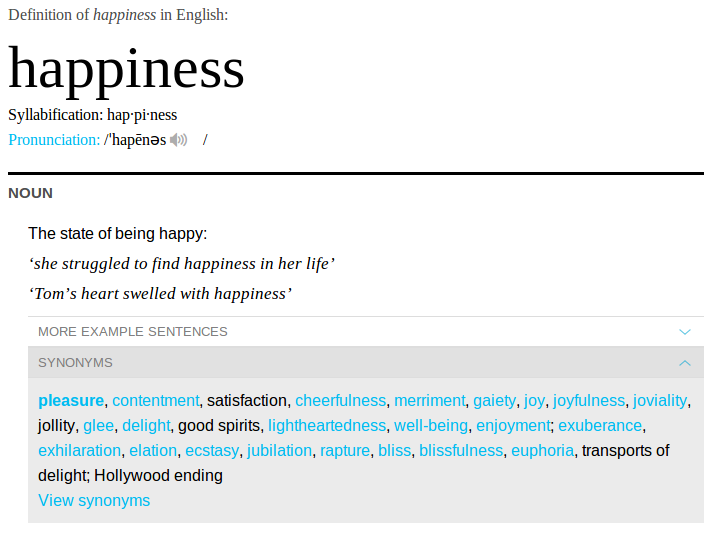
\includegraphics[width=.66\linewidth]{gfx/example-oxford-definition.png}}
        \caption{Entry example in the Oxford Dictionary online.}
        \label{fig:oxford-example}
\end{figure}

As one may notice in \autoref{fig:oxford-example}, the entry has many information: (i) the word itself, in ortographic form;
(ii) word syllabification; (iii) its pronunciation; (iv) the word audio file;
(v) \ac{POS} data; (vi) definition; (vii) some example sentences; (viii) and a list of synonyms. The pronunciation
follows Oxford's own transcription convention, which can be mapped on the \ac{IPA} as in \autoref{tab:oxford-dictionary-ipa}.

\renewcommand{\arraystretch}{0.8}% Tighter
\begin{table}[Hp]
\caption[Oxford Dictionary phone convention.]{Oxford Dictionary phone convention.}
\smallskip
\centering
\begin{tabular}{ccccc} \toprule
\tableheadline{\#} & \tableheadline{Oxford Phone} & \tableheadline{IPA Phone} & \tableheadline{Example} & \tableheadline{Transcription} \\ \midrule
1 & (h)w & \textipa{aaaaa} & when & trans \\ 
2 & \"a & \textipa{O} & hot & trans \\ 
3 & \^o & \textipa{O} & saw & trans \\ 
4 & \={oo} & \textipa{u} & too & trans \\ 
5 & \=a & \textipa{eI} & day & trans \\ 
6 & \=e & \textipa{i} & see & trans \\ 
7 & \=i & \textipa{aI} & my & trans \\ 
8 & \=o & \textipa{oU} & no & trans \\ 
9 & \textipa{@} & \textipa{@} & ago & trans \\ 
10 & \textipa{\oe} (foreign) & \textipa{\oe} & Goethe (German) & trans \\ 
11 & \textipa{\u{oo}} & \textipa{U} & put & trans \\ 
12 & \textipa{Y} (foreign) & \textipa{Y} & Utrecht (French) & trans \\ 
13 & a & \textipa{\ae} & cat & trans \\ 
14 & b & \textipa{b} & bad & trans \\ 
15 & CH & \textipa{tS} & chip  & trans \\ 
16 & d & \textipa{d} & day & trans \\ 
17 & e & \textipa{E} & bed & trans \\ 
18 & e(\textipa{@})r & \textipa{Er} & hair & trans \\ 
19 & f & \textipa{f} & fight & trans \\ 
20 & g & \textipa{g} & get & trans \\ 
21 & h & \textipa{h} & hi & trans \\ 
22 & i & \textipa{I} & sit & trans \\ 
23 & i(\textipa{@})r & \textipa{ir} & near & trans \\ 
24 & j & \textipa{dZ} & jar & trans \\ 
25 & k & \textipa{k} & kick & trans \\ 
26 & KH & \textipa{x} & loch & trans \\ 
27 & l & \textipa{l} & lie & trans \\ 
28 & m & \textipa{m} & man & trans \\ 
29 & N (foreign) & \textipa{\~v} & bon (French) & trans \\ 
30 & n & \textipa{n} & no & trans \\ 
31 & NG & \textipa{n} & ring & trans \\ 
32 & oi & \textipa{OI} & boy & trans \\ 
33 & ou & \textipa{aU} & how & trans \\ 
34 & p & \textipa{p} & pie & trans \\ 
35 & r & \textipa{r} & run & trans \\ 
36 & s & \textipa{s} & save & trans \\ 
37 & SH & \textipa{S} & she & trans \\ 
38 & t & \textipa{t} & time & trans \\ 
39 & TH & \textipa{D} & this & trans \\ 
40 & TH & \textipa{T} & thin & trans \\ 
41 & v & \textipa{v} & vow & trans \\ 
42 & y & \textipa{y} & yes & trans \\ 
43 & z & \textipa{z} & zoo & trans \\ 
44 & ZH & \textipa{Z} & decision & trans \\
\bottomrule
\end{tabular}
\label{tab:oxford-dictionary-ipa}
\end{table}
\renewcommand{\arraystretch}{1.0}% Normal

For compiling the corpus, we built a spider through Scrapy \cite{Scrapy2014}, a web crawling framework for Python specially 
designed to crawl websites and extract structured data from their pages. In total, $49,263$ entries were crawled. This number 
was defined in order to be consonant with the dictionary's legal aspects, which defines that only a fraction of its
content might be downloaded either personal or institutional use. For each word, we crawled three fields: the word, its transcription 
and the audio file. According to Oxford University Press' legal notice, we may not display or distribute any of the crawled 
content in any media, nor we may use commercially. Therefore, we used the data only for estimating the parameters of the acoustic model.

Some xenophones, i.e. phones from other languages, might be seen in \autoref{tab:oxford-dictionary-ipa}. This happens because
Oxford Dictionary also register some loanwords (specially those coming from Frech) with their original pronunciation,
like ``Utrecht'' and ``bon''. Since our goal is to deal only with Brazilian-accented English, words such as these
were excluded, so no word among the $49,263$ entries contain xenophones.

Oxford Dictionary's were recorded by many speakers (both male and female), with high-quality microphones, in sound-isolation rooms.
The audios are saved in MP3 format with \ac{VBR}, for this reason we had convert each file into WAV and downsample them to $16$ kHz.
The quality of the audio is excelent with a very high \ac{SNR}, as can be seen in the spectrogram for the word ``happiness''.

As one may observe in the regions of silence at the beginning and at the end of the utterance, the background noise approaches to zero.
A summary of the corpus can be seen in \autoref{fig:spectrogram-happiness}.

\begin{table}[H]
\caption[Summary of the Oxford Dictionary AmE Corpus.]{Summary of the Oxford Dictionary AmE Corpus.}
\smallskip
\centering
\begin{tabular}{ccc} \toprule
  Recorded files & 49,263 \\
  Total speech time & ~4 hours \\
  Average time per file & 1.02 seconds \\
  Original format & MP3 (VBR) \\
  Number of different speakers & Unknown \\
  \bottomrule
\end{tabular}
\label{tab:oxford-summary}
\end{table}

\clearpage
\subsubsection{Cambridge Dictionary}
Lorem ipsum quod dolor sit amet.

\subsubsection{OGI-22}
Lorem ipsum quod dolor sit amet.

\subsubsection{Westpoint}
Lorem ipsum quod dolor sit amet.

\subsubsection{LapsBM}
Lorem ipsum quod dolor sit amet.

\subsubsection{Youtube}
Lorem ipsum quod dolor sit amet.

\begin{table}[H]
\caption[Summary of Listener's Corpus.]{Summary of the Listener's Corpus.}
\smallskip
\centering
\begin{tabular}{ccc} \toprule
  Recorded files & 6,892 \\
  Total speech time & ~6.8 hours \\
  Average time per file & 1.02 seconds \\
  Original format & WAV 16kHz \\
  Number of different speakers & 53 \\
  \bottomrule
\end{tabular}
\end{table}


\clearpage
\subsection{Building the Acoustic Model}

\subsubsection{The Phoneset}\label{sec:listener-phoneset}

Since our goal is to build an \ac{ASR} system capable of recognizing non-native speech, we propose
to use an interlingual phoneset as the basis of the pronunciation model. By doing this, we can define
\ac{HMM} models for estimating phones which are part of both the speaker's native language (\ac{BP}) and 
the target language (\ac{AmE}).

A straightforward approach would be to look up the literature in phonetics and phonology in order to find
a \ac{BP}--\ac{AmE} interlingual phoneset. However, to the best of our knowledge, no previous works were carried 
out in this regard. There are papers addressing specific mispronunciations, such as those discussed in \autoref{sec:common-mispronunciation}, 
which list some occurring interlingual phones, but there is not a wide-ranging study available about this matter.

Therein we had to develop our own interlingual phoneset. For simplicity, we decided to adapt the union set formed 
by the phones contained in two machine-readable dictionaries, one for \ac{AmE}: \ac{CMUdict} \cite{CMU2008}, and another for \ac{BP}: 
Aeiouad\^o \cite{Mendonca2014}. By doing this, we can cover most of the phone productions that brazilian \ac{ESL} learners are likely
to make. Advanced students will tend to use more properly the English phones, whereas beginners will have a stronger accent,
thus producing more phones from the \ac{BP} phoneset. A brief description of each of these dictionaries is given below, before 
we go into further details of our interlingual set.

\ac{CMUdict} \citep{CMU2008} is a machine-readable pronunciation dictionary for \ac{AmE} which has about $125,000$ 
words and their transcriptions. It was designed primarily for speech applications, such as speech recognition and synthesis, 
and it has been widely tested in both Academia and industry.

Words in \ac{CMUdict} are transcribed using ARPAbet, a phonetic transcription code developed by the Advanced Research Projects Agency in 
$1971$. It represents each \ac{AmE} phone with a distinct sequence of \ac{ASCII} characters. In the dictionary, there are in total $39$ 
phones plus stress marks. The phone convention is described on \autoref{tab:cmu-conv}.

\renewcommand{\arraystretch}{0.95}% Tighter
\begin{table}[p]
\caption[CMUdict phone convention.]{CMUdict phone convention.}
\smallskip
\centering
\begin{tabular}{ccccc} \toprule
\tableheadline{\#} & \tableheadline{CMU Phone} & \tableheadline{IPA Phone} & \tableheadline{Example} & \tableheadline{Transcription} \\ \midrule
1 & AA & [\textipa{A}] & odd & AA D \\
2 & AE & [\textipa{\ae}] & at & AE T \\
3 & AH & [\textipa{@}] & hut & HH AH T \\
4 & AO & [\textipa{O}] & ought & AO T \\
5 & AW & [\textipa{aU}] & cow & K AW \\
6 & AY & [\textipa{aI}] & hide & HH AY D \\
7 & B & [\textipa{b}] & be & B IY \\
8 & CH & [\textipa{tS}] & cheese & CH IY Z \\
9 & D & [\textipa{d}] & dee & D IY \\
10 & DH & [\textipa{D}] & thee & DH IY \\
11 & EH & [\textipa{E}] & Ed & EH D \\
12 & ER & [\textipa{@r}] & hurt & HH ER T \\
13 & EY & [\textipa{A\*r}] & ate & EY T \\
14 & F & [\textipa{f}] & fee & F IY \\
15 & G & [\textipa{g}] & green & G R IY N \\
16 & HH & [\textipa{h}] & he & HH IY \\
17 & IH & [\textipa{I}] & it & IH T \\
18 & IY & [\textipa{i}] & eat & IY T \\
19 & JH & [\textipa{dZ}] & gee & JH IY \\
20 & K & [\textipa{k}] & key & K IY \\
21 & L & [\textipa{l}] & lee & L IY \\
22 & M & [\textipa{m}] & me & M IY \\
23 & N & [\textipa{n}] & knee & N IY \\
24 & NG & [\textipa{N}] & ping & P IH NG \\
25 & OW & [\textipa{oU}] & oat & OW T \\
26 & OY & [\textipa{OI}] & toy & T OY \\
27 & P & [\textipa{p}] & pee & P IY \\
28 & R & [\textipa{\*r}] & read & R IY D \\
29 & S & [\textipa{s}] & sea & S IY \\
30 & SH & [\textipa{S}] & she & SH IY \\
31 & T & [\textipa{t}] & tea & T IY \\
32 & TH & [\textipa{T}] & theta & TH EY T AH \\
33 & UH & [\textipa{U}] & hood & HH UH D \\
34 & UW & [\textipa{u}] & two & T UW \\
35 & V & [\textipa{v}] & vee & V IY \\
36 & W & [\textipa{w}] & we & W IY \\
37 & Y & [\textipa{y}] & yield & Y IY L D \\
38 & Z & [\textipa{z}] & zee & Z IY \\
39 & ZH & [\textipa{Z}] & seizure & S IY ZH ER \\
\bottomrule
\end{tabular}
\label{tab:cmu-conv}
\end{table}
\renewcommand{\arraystretch}{1.0}% Normal

As for Aeiouad\^o, as described in Section~\autoref{sec:aeiouado}, its transcriptions are
based on the dialect of S\~ao Paulo city and contains 39 different phones. The dictionary makes
use of a hybrid approach for converting graphemes into phonemes, 
which employs both manual transcription rules and machine learning algorithms. Its phone convention
is presented in Table~\autoref{tab:aeiouado-conv}.

\renewcommand{\arraystretch}{0.9}% Tighter
\begin{table}[p]
\caption[Aeiouad\^o phone convention.]{Aeiouad\^o phone convention.}
\smallskip
\centering
\begin{tabular}{ccccc} \toprule
\tableheadline{\#} & \tableheadline{Aeiouad\^o Phone} & \tableheadline{IPA Phone} & \tableheadline{Example} & \tableheadline{Transcription} \\ \midrule
1 & a & [\textipa{a}] & amor & a m o x \\
2 & a$\sim$ & [\textipa{\~a}] & canto & k a$\sim$ t U \\
3 & b & [\textipa{b}] & besta & b e s t @ \\
4 & d & [\textipa{d}] & da & d a \\
5 & dZ & [\textipa{dZ}] & dia & dZ i @ \\
6 & E & [\textipa{E}] & \'e & E \\
7 & e & [\textipa{e}] & dedo & d e d U \\
8 & e$\sim$ & [\textipa{\~e}] & venda & v e$\sim$ d @ \\
9 & f & [\textipa{f}] & frio & f 4 i U \\
10 & g & [\textipa{g}] & gula & g u l @  \\
11 & G & [\textipa{G}] & carga & carga \\
12 & i & [\textipa{i}] & a\'i & a i \\
13 & I & [\textipa{I}] & come & k o$\sim$ m I \\
14 & i$\sim$ & [\textipa{\~i}] & sim & s i$\sim$ \\
15 & J & [\textipa{\textltailn}] & ganho & g a$\sim$ J U \\
16 & j & [\textipa{y}] & pai & p a j \\
17 & j$\sim$ & [\textipa{\~y}] & parem & p a 4 e$\sim$ j$\sim$ \\
18 & k & [\textipa{k}] & compra & k o$\sim$ p 4 @ \\
19 & l & [\textipa{l}] & l\'a & l a \\
20 & L & [\textipa{L}] & palha & p a L @ \\
21 & m & [\textipa{m}] & m\~ae & m a$\sim$ j$\sim$ \\
22 & n & [\textipa{n}] & n\~ao & n a$\sim$ w$\sim$ \\
23 & O & [\textipa{O}] & p\'o & p O \\
24 & o & [\textipa{o}] & gorro & g o x U \\
25 & o$\sim$ & [\textipa{\~o}] & com & k o$\sim$ \\
26 & p & [\textipa{p}] & pessoa & p e s o @ \\
27 & s & [\textipa{s}] & susto & s u s t U \\
28 & s & [\textipa{S}] & chato & S a t U \\
29 & t & [\textipa{t}] & tato & t a t U \\
30 & tS & [\textipa{tS}] & noite & n o j tS I \\
31 & u & [\textipa{u}] & durmo & d u G m U \\
32 & U & [\textipa{U}] & c\'umulo & k u m u l U \\
33 & u$\sim$ & [\textipa{\~u}] & um & u$\sim$ \\
34 & v & [\textipa{v}] & vida & v i d @ \\
35 & w & [\textipa{w}] & aula & a w l @ \\
36 & w$\sim$ & [\textipa{\~w}] & canh\~ao & k a$\sim$ J a$\sim$ w$\sim$ \\
37 & x & [\textipa{x}] & rato & x a t U \\
38 & z & [\textipa{z}] & zebra & z e b 4 @ \\
39 & 4 & [\textipa{R}] & arara & a 4 a 4 @ \\
40 & @ & [\textipa{@}] & bola & b O l @ \\
\bottomrule
\end{tabular}
\label{tab:aeiouado-conv}
\end{table}
\renewcommand{\arraystretch}{1.0}% Normal

In what concerns to our interlingual phoneset, we kept all \ac{CMUdict} phones, since that is the target language's
phoneset the learners are trying to achieve. Then we compared each phone in \ac{CMUdict} with those contained in 
Aieouad\^o, in order to check for missing phones and to analyze whether the overlapping ones really correspond to the same
sound.

At a first glance, it seems that \ac{BP} and \ac{AmE} share a pool of 24 common phones, comprising fifteen consonantes
[\textipa{b}, \textipa{d}, \textipa{dZ}, \textipa{f}, \textipa{g}, 
\textipa{k}, \textipa{l}, \textipa{m}, \textipa{n}, \textipa{p}, \textipa{s}, \textipa{S}, \textipa{t}, \textipa{tS}, \textipa{v}, \textipa{z}];
seven vowels [\textipa{E}, \textipa{i}, \textipa{I}, \textipa{O}, \textipa{u}, \textipa{U}, \textipa{@}];
together with two glides [\textipa{y}, \textipa{w}]. However it is worth noticing that this first impression does not
hold true. 

Despite the fact that both dictionaries present \ac{IPA} correspondences, such correspondes should not be taken
for granted, without previous analysis. In theory, \ac{IPA} is capable of describing any sound produced by the human vocal 
tract with exactness. Still \ac{IPA} transcriptions are biased by the level of detail one wishes to express and by the 
assumptions of the transcriber. This is the case for some of these overlapping phones. Several of these consonants and vowels, 
although marked with the same \ac{IPA} symbol by \ac{CMUdict} and Aeiouad\^o,
in fact, can not be regarded as being the same sound, since they show a very different distribution
in English and \ac{BP}. 

For instance, the production of /\textipa{p}, \textipa{t}, \textipa{k}/, 
in \ac{BP} and \ac{AmE} can be quite different. In English, such consonants are generally produced as 
[\textipa{p}, \textipa{t}, \textipa{k}]. However it is known that when they occur in certain contexts, 
for example, in word initial position or onset of a stressed syllable, they become aspirated; whence
[\textipa{p\super h}, \textipa{t\super h}, \textipa{k\super h}] \citep{Lisker1985}. 
On the other hand, this process is not found in \ac{BP}, where, disregard of the context, [\textipa{p}, \textipa{t}, \textipa{k}] show no 
relevant levels of aspiration \citep{Klein1999}. 

For that reason, in order to properly estimate the \ac{HMM} states for the interlingual phones, it is mandatory
to create aspirated phone models for these consonants that are different from the non-aspirated ones. In our interlingual
phoneset, we decided to keep the distinction between aspirated and non-aspirated phones. Therefore, according to our
convention, the /\textipa{p}/ that occurs in a stressed syllable of an English word like ``pie'' is transcribed as [\textipa{p\super h}], 
while the /\textipa{p}/ of an unstressed syllable or a BP word is transcribed as [\textipa{p}]. 

Additionally, some vowels that are described by both dictionaries with the same \ac{IPA} symbol are not exactly equal.
Although English and \ac{BP} both possess the vowels [\textipa{I, @, U}], the distribution
of these phones between both languages is fairly different. In \ac{AmE} such vowels hold phonological status, i.e. they 
are phonemes, so that one could find minimal pairs differing only by [\textipa{I, @, U}], such as ``sheep'' [\textipa{"Sip}] vs. 
``ship'' [\textipa{"SIp}]; ``cut'' [\textipa{"k\super h@t}] vs. ``cat'' [\textipa{"k\super h\ae t}]; and ``pull'' 
[\textipa{"p\super hUl}] vs. pool [\textipa{"p\super hul}]. As for \ac{BP}, these vowels exist solely as part
of a phonological process. When the tense vowels [\textipa{i, a, u}] occur in unstressed word-final position, they undergo a lenition process
and are produced as the lax vowels [\textipa{I, @, U}], respectivelly. Hence the \ac{BP} [\textipa{I, @, U}] have 
different formant values \cite{Fails1992} and all the typical characteristics of lax vowels, that is, they are short, 
they have less energy and, consequently, less clear-cut formants \cite{Nobre1987}.

With regard to the missing phones, there were 15 phones which are only present in the \ac{BP} inventory, these include eight vowels
[\textipa{a}, \textipa{\~a}, \textipa{e}, \textipa{\~e}, \textipa{\~i}, \textipa{o}, \textipa{\~o}, \textipa{\~u}]; five
consonants [\textipa{G}, \textipa{\textltailn}, \textipa{L}, \textipa{x}, \textipa{R}]; and two nasal glides
[\textipa{\~y}, \textipa{\~w}]. 

All eight vowels were added to the interlingual phoneset, for they encompass negative transfer problems. For instance, 
[\textipa{\~a}, \textipa{\~e}, \textipa{\~i}, \textipa{\~o}, \textipa{\~u}] are related to
vocalization of final nasals (\emph{vide} \ref{sec:voc-nasals}) and [\textipa{a}, \textipa{e}, \textipa{o}] to vowel assimilation (\emph{vide} \ref{sec:voc-assimilation}).

The \ac{BP} rhotic consonants [\textipa{R}, \textipa{G}, \textipa{x}], were merged onto the same sound, [\textipa{h}] owing to the fact
they they represent \ac{BP} dialectal variants not relevant to L1-L2 interphonology.

Furthermore, the \ac{BP} palatal consonants [\textipa{\textltailn}, \textipa{L}] were not considered in the final interlingual phoneset,
since we could not find, in the literature, any negative transfer process in which they occur. 

The nasal glides were excluded from the interlingual phoneset, instead we preffered to combine them with their accompanying vowels, in
order to create nasal diphthongs, such as [\textipa{\~a\~I}, \textipa{\~a\~U}, \textipa{\~e\~I}, \textipa{\~o\~I}]. This decision was 
made in accordance with \cite{Demasi2010}, which found that \ac{BP} nasal diphthongs have a very particular behavior, with 
articulatory, acoustic and aerodynamic patterns different from the non-nasalized ones. 
We believe that a single \ac{HMM} model for each diphthong will be able to better gauge this behavior.

The final phoneset, which we used as the basis for our \ac{ASR} system, can be found in \autoref{tab:interlingual-conv}.

\renewcommand{\arraystretch}{0.6}% Tighter

\begin{table}[p]
\caption[Interlingual dictionary phone convention.]{Interlingual dictionary phone convention. BP word examples are shown in \emph{italics}.}
\smallskip
\centering
\begin{tabular}{ccccc} \toprule
\tableheadline{\#} & \tableheadline{Interl. Phone} & \tableheadline{IPA Phone} & \tableheadline{Example} & \tableheadline{Transcription} \\ \midrule
 1 & \small a & \small  [\textipa{@}] & \small \emph{da} & \small d a \\ 
\small 2 & \small aa & \small  [\textipa{A}] & \small odd & \small aa d \\ 
\small 3 & \small aaa & \small  [\textipa{a}] & \small \emph{d\'a} & \small d aaa \\ 
\small 4 & \small ae & \small  [\textipa{\ae}] & \small cat & \small k ae t \\ 
\small 5 & \small ah & \small  [\textipa{@}] & \small but & \small b ah t \\ 
\small 6 & \small ahw & \small  [\textipa{@U}] & \small xxx & \small xx xx \\ 
\small 7 & \small am & \small  [\textipa{\~a}] & \small xxx & \small xx xx \\ 
\small 8 & \small ao & \small  [\textipa{O}] & \small for & \small f ao r \\ 
\small 9 & \small aow & \small [\textipa{OU}] & \small xxx & \small xx xx \\ 
\small 10 & \small aw & \small [\textipa{aU}] & \small cow & \small k aw \\ 
\small 11 & \small awm & \small [\textipa{\~a\~U}] & \small \emph{n\~ao} & \small n awm \\ 
\small 12 & \small ay & \small [\textipa{aI}] & \small I & \small ay \\ 
\small 13 & \small aym & \small [\textipa{\~a\~I}] & \small m\~ae & \small m aym \\ 
\small 14 & \small b & \small [\textipa{b}] & \small boot & \small b uw tt \\ 
\small 15 & \small ch & \small [\textipa{tS}] & \small cheek & \small ch iy kk \\ 
\small 16 & \small d & \small [\textipa{d}] & \small do & \small d uw \\ 
\small 17 & \small dh & \small [\textipa{D}] & \small that & \small dh ae tt \\ 
\small 18 & \small e & \small [\textipa{e}] & \small \emph{eu} & \small e w \\ 
\small 19 & \small eh  & \small [\textipa{E}] & \small merry & \small m eh r iy \\ 
\small 20 & \small em & \small [\textipa{\~e}] & \small \emph{entendi} & \small em tt em jh i \\ 
\small 21 & \small ey & \small [\textipa{eI}] & \small April & \small ey pp r iy ll \\ 
\small 22 & \small eym & \small [\textipa{\~e\~I}] & \small \emph{hein} & \small eym \\ 
\small 23 & \small f & \small [\textipa{f}] & \small fat & \small f ae tt \\ 
\small 24 & \small g & \small [\textipa{g}] & \small guy & \small g ay \\ 
\small 25 & \small hh & \small [\textipa{h}] & \small heat & \small hh iy tt  \\ 
\small 26 & \small ih & \small [\textipa{I}] & \small bit & \small b ih tt \\ 
\small 27 & \small i & \small [\textipa{I}] & \small \emph{comi} & \small k o m i \\ 
\small 28 & \small im & \small [\textipa{\~i}] & \small \emph{sim} & \small s im \\ 
\small 29 & \small iy & \small [\textipa{i}] & \small eat & \small iy tt \\ 
\small 30 & \small jh & \small [\textipa{dZ}] & \small judge & \small jh ah jh \\ 
\small 31 & \small k & \small [\textipa{k\super h}] & \small cool & \small k uw ll \\ 
\small 32 & \small kk & \small [\textipa{k}] & \small cai & \small kk ay \\ 
\small 33 & \small l & \small [\textipa{l}] & \small lounge & \small l aa uh n jh \\ 
\small 34 & \small ll & \small [\textipa{l\super G}] & \small fall & \small f ao ll \\ 
\small 35 & \small m & \small [\textipa{m}] & \small mother & \small m ah dh ah r \\ 
\small 36 & \small n & \small [\textipa{n}] & \small neat & \small n iy tt \\ 
\small 37 & \small ng & \small [\textipa{N}] & \small king & \small k ih ng \\ 
\small 38 & \small o & \small [\textipa{o}] & \small s\^o & \small s o \\ 
\small 39 & \small om & \small [\textipa{\~o}] & \small \emph{conto} & \small kk om tt u\\ 
\small 40 & \small ow & \small [\textipa{oU}] & \small no & \small n ow \\ 
\small 41 & \small ohy & \small [\textipa{OI}] & \small boys & \small b oy z\\ 
\small 42 & \small oym & \small [\textipa{\~o\~I}] & \small \emph{doa\c{c}\~oes} & \small d o a s oym s\\ 
\small 43 & \small p & \small [\textipa{p\super h}] & \small pity & \small p ih rd iy \\ 
\small 44 & \small pp & \small [\textipa{p}] & \small \emph{pai} & \small pp ay \\ 
\small 45 & \small r & \small [\textipa{r}] & \small run & \small r ah n \\ 
\small 46 & \small rd & \small [\textipa{R}] & \small city & \small s ih rd iy \\ 
\small 47 & \small s & \small [\textipa{s}] & \small six & \small s ih k s \\ 
\small 48 & \small sh & \small [\textipa{S}] & \small shoes & \small sh uw z \\ 
\small 49 & \small t & \small [\textipa{t\super h}] & \small time & \small t ay m \\ 
\small 50 & \small th & \small [\textipa{T}] & \small three & \small th r iy \\ 
\small 51 & \small tt & \small [\textipa{t}] & \small \emph{tudo} & \small tt uw d u \\ 
\small 52 & \small u & \small [\textipa{U}]  & \small \emph{como} & \small kk om m u \\ 
\small 53 & \small uh & \small [\textipa{U}] & \small could & \small k uw d \\ 
\small 54 & \small um & \small [\textipa{\~u}] & \small \emph{rum} & \small hh um \\ 
\small 55 & \small uw & \small [\textipa{u}] & \small wood & \small w uw d \\ 
\small 56 & \small v & \small [\textipa{v}] & \small van & \small v ae n \\ 
\small 57 & \small w & \small [\textipa{w}] & \small what & \small w aa tt \\ 
\small 58 & \small y & \small [\textipa{y}] & \small union & \small y uw n y ah n \\ 
\small 59 & \small z & \small [\textipa{z}] & \small zoo & \small z uw \\ 
\small 60 & \small zh & \small [\textipa{Z}] & \small leisure & \small l eh zh ah r \\ 
\bottomrule
\end{tabular}
\label{tab:interlingual-conv}
\end{table}
\renewcommand{\arraystretch}{1.0}% Normal

\clearpage
\subsubsection{Speech Data}

Many of the 



\subsubsection{HMM topology}

\subsubsection{Tree-Based State Tying}

Data-driven approaches also show limitations. Since such approaches are generally based on 
the positive examples which occur in a corpus, rare or non-occuring phenomena are often poorly estimated or even neglected.
This is the case for triphone \ac{HMM} models. 

Natural languages have, on average, $30$ different phones. The language believed to have the smallest phonetic inventory is 
Rotokas (East Papuan, New Guinea), with 11 phones, and the one with largest is !X\'o\~o  (Khoisan, Botswana/Namibia), 
with 160 \citep{Hayes2011}. English is usually assumed to have 37 to 41 phones, depending on the dialect. 

In the \ac{CMUdict} \citep{CMU2008}, 39 phones are used to describe the words of \ac{AmE}. When it comes to triphones, in theory, 
this number might grow by three orders of magnitude, that is $39^3$ or $59,319$. It is true that due to phonotactic constraints
many of the virtually possible triphones never take place in practice. 
For instance, the triphone sequence [\textipa{N}-\textipa{s}+\textipa{p}] does not exist in English, although it 
is made of valid and existing monophones [\textipa{N}], [\textipa{s}] and [\textipa{p}]. 

\citeauthor{Kuperman2008} \citep{Kuperman2008} examined the monophone, diphone and triphone frequencies in speech corpora
for many languages. In what concerns to English, they analysed the Buckeye Corpus and reported that it contains $29,804$ different 
occurring triphones (or types), distributed among $431,000$ tokens. Although the actual number of triphones for English is
almost half the number of possible permutations, it is still a huge number of triphones to model over a corpus. 
Therefore, in order to build an \ac{ASR} system, one always has to deal with data scarcity and try to overcome its limitations.

Within \ac{HMM} \ac{ASR}, tree-based state tying is a technique to improve the modelling of rare triphones and allow the 
estimation of non-occurring ones. It was initially proposed by \citeauthor{Young1994} \citep{Young1994} and since then
has become a standard procedure in \ac{HMM} \ac{ASR} systems. The aim of tree-based state tying is to maintain the balance 
between the model complexity and the available training data by tying the \ac{HMM} states of acoustically similar triphones.

In contrast to the majority of methods in \ac{ASR}, tree-based state tying is carried out in a top-down, knowledge-based 
way. A specialist (generally a speech sciencist, phologist or phoneticist) uses his/her knowledge to build a phonetic decision 
tree which will organize the phones into sets with similar acoustic parameters. 

In most cases, the criteria used to organize phones into a decision tree are the so-called natural classes. 
Natural classes were proposed within the generative phonology framework. In this framework, phones and and phonemes are no 
longer considered the basic units of analysis, instead it is assumed that they can be broken down into smaller components,
which describe aspects of articulation and perception, such as [+nasal], [-continuant], [+strident], etc. For instance,
the phone [\textipa{s}] would not be represented in generative phonology as a single phonetic symbol [\textipa{s}], but 
as a bundle of distinctive features \citep{Jensen2004}:
\[
[{\textipa{a}}] \rightarrow 
\begin{bmatrix}
+consonantal \\ -syllabic \\ -sonorant \\ +continuant \\ +anterior \\ +coronal \\ +strident \\ -voiced
\end{bmatrix}
\]

Distinctive features were probably the most important contribution of generative phonology. They became popular as a
model specially because they were able of simplify phonological processes by grouping segments. Consider the case of
final-obstruent devoicing. In many pronunciations of Standard German, voiced obstruent consonants become devoiced when
they occur in word final position. This is the case for a large number of german nouns which make their plural by the 
addition of the suffix \{-\textipa{e}\}. \autoref{tab:german-devoicing} contains a few examples extracted from 
\citeauthor{Grijzenhout2000} \citep{Grijzenhout2000}.

\begin{table}[H]
\caption[Examples of final-obstruent devoicing in German.]{Examples of final-obstruent devoicing in German.}
\smallskip
\centering
\begin{tabular}{ccc} \toprule
  \tableheadline{Plural form} & \tableheadline{Singular form} & \tableheadline{Gloss} \\ \midrule
  Hun[\textipa{d}]e & Hun[\textipa{t}] & \small{dog} \\
  Die[\textipa{b}]e & Die[\textipa{p}] & \small{thief} \\
  Ber[\textipa{g}]e & Ber[\textipa{k}] & \small{mountain} \\
  M\"au[\textipa{z}] & Mau[\textipa{s}] & \small{mouse} \\
  \bottomrule
\end{tabular}
\label{tab:german-devoicing}
\end{table}

As one can observe at the provided examples, the plural forms contain only voiced obstruents whilst the singular forms contain their 
devoiced counterparts. To express this phonological process within structural phonology, one would have to introduce at
least four rules:
\[
[\textipa{b}] \rightarrow [\textipa{p}]  / \_ \# 
\]
\[
[\textipa{d}] \rightarrow [\textipa{t}]  / \_ \#
\]
\[
[\textipa{g}] \rightarrow [\textipa{k}]  / \_ \#
\]
\[
[\textipa{d}] \rightarrow [\textipa{s}]  / \_ \#
\]

Whereas using distinctive features, all cases of german final-obstruent devoicing can be explained by a single rule:
\[
\begin{bmatrix}
+consonantal \\ -syllabic \\ -sonorant \\ +voiced
\end{bmatrix} \rightarrow 
\begin{bmatrix}
-voiced
\end{bmatrix}
 / \_ \#
\]

The main benefits of distinctive features lie in their capability of making generalizations, that is to say
of grouping phones together in a meningful way.  Phonologists have long known that sounds that share the same manner, 
place of articulation, or voicing level behave similarly. Distinctive features provide a way to express this
in an elegant way, by stablishing that feature matrices which are not fully specified do form a natural class. 
Therefore a distinctive features matrix
\[
\begin{bmatrix}
+consonantal \\ -syllabic
\end{bmatrix}
\]
represents all consonants, whereas
\[
\begin{bmatrix}
+consonantal \\ -syllabic \\ +continuant \\ +voiced
\end{bmatrix}
\]
represents all voiced fricatives, etc. For developing the phonetic decision tree, the specialist employs his/her 
knowledge of phonetics and phonology in order to define questions about the phonetic environment of a given 
phone. This phonetic environment is defined by using natural classes, such that an example question would
be ``is the phone preceded by an obstruent?'' or ``is there a fricative after the phone?'' Technically, the tree is a 
binary one, i.e a connected acyclic graph such that the degree of each vertex is no more than three. Each
internal node of the tree represents a question about the phonetic context a triphone, each branch represents the answer in a yes-no
form and leaf nodes define \ac{HMM} states. Once the tree is built, its structure is used to decide how \ac{HMM} states will
be tied among triphone models. \autoref{fig:decision-tree} presents an example of a phonetic decision tree.

\begin{figure}[H]
        \myfloatalign
        {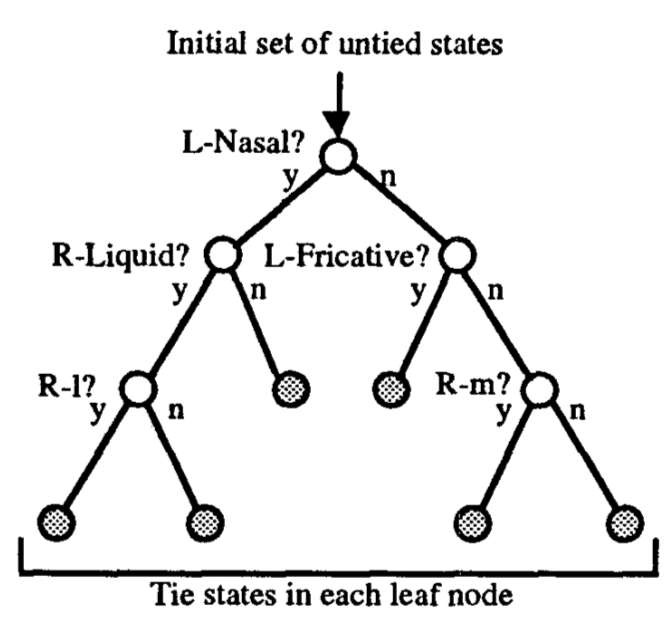
\includegraphics[width=.66\linewidth]{gfx/decision-tree.png}}
        \caption{Phonetic decision tree for HMM state tying \citep{Young1994}.}
        \label{fig:decision-tree}
\end{figure}

The tree input is each triphone being analysed.

The clustering procedures begins by placing all observations in a single root node. All questions are 
analised and the one which maximise the likelihood of a single diagonal
covariance Gaussian is chosen, then the node is split and child nodes generated. The splitting goes on
until it falls below a threshold. Commonly, a minimum threshold is also set, the usual approach is to consider
the frequency of occurence of the phones in a corpus. That it, if a given phone $p$ has $m$ samples and the minimum
threshold is $m$, such that $m>n$, the phone $p$ is mapped unto a more general and robust phone. Consider
that the triphone \textipa{[I-N+g]} appeared 30 times on corpus, and the minimum threshold for splitting the node
was $45$, then \textipa{[I-N+g]} would be modeled into a more general phone, say, for instance, [\textipa{i-N+g}] or 
[\textipa{i-N}].

In the example shown in \autoref{fig:decision-tree}, the first node 
(the root of the tree) checks if the left part of the triphone contains a nasal consonant. If positive, the tree 
examines the right side of the triphone, by questioning
whether it is a liquid consonant. If negative, a leaf is reached and the HMM state to be tied is outputted, e.g. ``tie
the 1\textsuperscript{st} emitting HMM state of the analysed triphone $A$ to [Nasal-$A$+*]''. 
\autoref{fig:state-tying-tree} summarizes the state tying procedure.

\begin{figure}[H]
        \myfloatalign
        {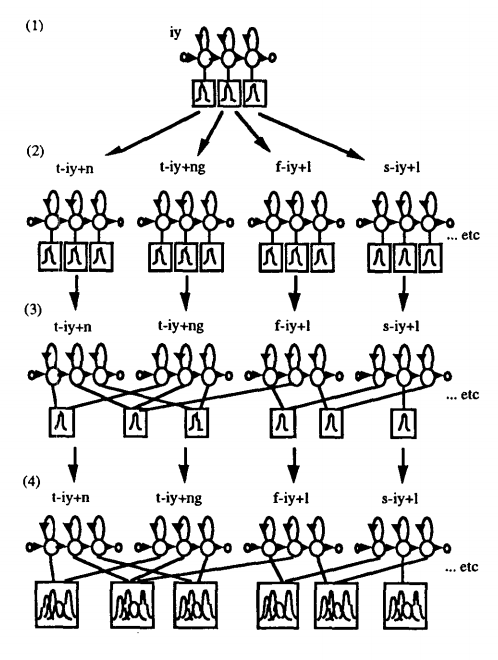
\includegraphics[width=.66\linewidth]{gfx/state-tying-tree.png}}
        \caption{Tied-state HMM system build procedure \citep{Young1994}.}
        \label{fig:state-tying-tree}
\end{figure}

For building the phonetic decision tree for Listener, we based ourselves on the distinctive feature set proposed by 
\citeauthor{Jensen2004} \citep{Jensen2004}, which follows the main guidelines of generative phonology by dividing
the features into four central classes: i) major class features, ii) manner features; iii) place features; and 
iv) laryngeal features.

In practice, classes work as following. Major class features distinguish among the most general classes of sound, 
i.e. vowels, consonants and glides (or semi-vowels). Manner features determine how sounds are articulated, 
that is do they consist of a stop, a nasal, a fricative, a liquid, a trill or a flap? Place features describe 
where in the mouth sounds are produced, whether in the labial region, the alveolar region, the velar region, etc.
Finally, laryngeal features represent the glottal states of sounds, their basic purpose is to differ voiced 
sounds from unvoiced ones.

\citeauthor{Jensen2004} \citep{Jensen2004} proposes a set of $17$ features to describe most of the world languages.

\begin{enumerate}
 \item \emph{Major class features}: syllabic, consonantal and sonorant;
 \item \emph{Manner features}: continuant, nasal, lateral, strident and delayed release;
 \item \emph{Place features}: anterior, coronal, distributed, high, low, back, round and \ac{ATR}.
 \item \emph{Laryngeal features}: voice and \ac{HSP};
\end{enumerate}

The somewhat reduced set for place features is capable of representing a large amount of places of articulation 
since features which are regularly restricted to vowels (such as high, low, back and round) are also shared 
with consonants. Besides, once features have a binary nature, therefore, in theory, a number $n$ of features is able
to dintinguish up to $2^n$ phones. In \autoref{fig:features-place}, a comparison is shown between place features and their corresponding
regions of articulation. For a full explanation of each feature, please see \citeauthor{Jensen2004} \citep{Jensen2004}.

\begin{figure}[H]
        \myfloatalign
        {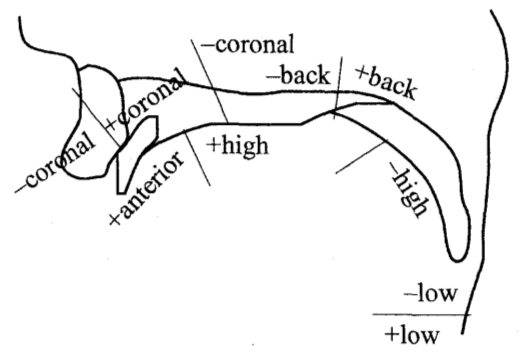
\includegraphics[width=.66\linewidth]{gfx/features-place.png}}
        \caption{Distinctive features for places of places of articulation \citep{Jensen2004}.}
        \label{fig:features-place}
\end{figure}

According to this set of distinctive features, we can arrange the entire phonetic inventory of \ac{AmE} as in \autoref{tab:dist-features-eng}
and that of \ac{BP} as in \autoref{tab:dist-features-bp}.

\tabcolsep=0.15cm
\begin{table}[htbp]
\caption{Distinctive features chart for AmE phones \citep{Jensen2004}.}
\begin{center}
\begin{tabular}{|cc|cccccccccccccccccc|}\hline
 &  & \multicolumn{18}{c|}{\textsc{Distinctive features}} \\ \cline{3-20}
\rotatebox[origin=c]{90}{\textsc{\textsc{CMU symbol}}} & \rotatebox[origin=c]{90}{\textsc{\textsc{IPA symbol}}} & \rotatebox[origin=c]{90}{\textsc{\textsc{syllabic}}} & \rotatebox[origin=c]{90}{\textsc{consonantal}} & \rotatebox[origin=c]{90}{\textsc{sonorant}} & \rotatebox[origin=c]{90}{\textsc{voice}} & \rotatebox[origin=c]{90}{\textsc{HSP}} & \rotatebox[origin=c]{90}{\textsc{continuant}} & \rotatebox[origin=c]{90}{\textsc{nasal}} & \rotatebox[origin=c]{90}{\textsc{lateral}} & \rotatebox[origin=c]{90}{\textsc{strident}} & \rotatebox[origin=c]{90}{\textsc{del. release}} & \rotatebox[origin=c]{90}{\textsc{anterior}} & \rotatebox[origin=c]{90}{\textsc{coronal}} & \rotatebox[origin=c]{90}{\textsc{  distributed  }} & \rotatebox[origin=c]{90}{\textsc{high}} & \rotatebox[origin=c]{90}{\textsc{low}} & \rotatebox[origin=c]{90}{\textsc{back}} & \rotatebox[origin=c]{90}{\textsc{ATR}} & \rotatebox[origin=c]{90}{\textsc{round}} \\ \hline
AA & [\textipa{A}] & + & - & + & + & - & + & - & - & - & - & - & - & - & - & + & + & + & - \\[-3.5pt]
AE & [\textipa{ae}] & + & - & + & + & - & + & - & - & - & - & - & - & - & - & + & - & - & - \\[-3.5pt]
AH & [\textipa{@}] & + & - & + & + & - & + & - & - & - & - & - & - & - & - & - & + & - & - \\[-3.5pt]
AO & [\textipa{O}] & + & - & + & + & - & + & - & - & - & - & - & - & - & - & + & + & - & + \\[-3.5pt]
AW & [\textipa{aU}] & + & - & + & + & - & + & - & - & - & - & - & - & - & - & - & - & - & - \\[-2pt] \hline
AY & [\textipa{aI}] & + & - & + & + & - & + & - & - & - & - & - & - & - & - & - & - & - & - \\[-3.5pt]
B & [\textipa{b}] & - & + & - & + & - & - & - & - & - & - & + & - & - & - & - & - & - & - \\[-3.5pt] 
CH & [\textipa{tS}] & - & + & - & - & - & - & - & - & + & + & - & - & - & - & - & - & - & - \\[-3.5pt] 
D & [\textipa{d}] & - & + & - & + & - & - & - & - & - & - & + & + & - & - & - & - & - & - \\[-3.5pt] 
DH & [\textipa{D}] & - & + & - & + & - & + & - & - & - & - & + & + & - & - & - & - & - & - \\[-2pt] \hline
EH & [\textipa{E}] & + & - & - & + & - & + & - & - & - & - & - & - & - & - & - & - & - & - \\[-3.5pt] 
EY & [\textipa{A\*r}] & + & - & + & + & - & + & - & - & - & - & - & - & - & - & - & - & + & - \\[-3.5pt] 
F & [\textipa{f}] & - & + & - & - & - & + & - & - & - & - & + & - & - & - & - & - & - & - \\[-3.5pt] 
G & [\textipa{g}] & - & + & - & + & - & - & - & - & - & - & - & - & - & - & - & - & - & - \\[-3.5pt] 
HH & [\textipa{h}] & - & + & - & - & - & + & - & - & - & - & - & - & + & - & - & - & - & - \\[-2pt] \hline
IH & [\textipa{I}] & + & - & + & + & - & + & - & - & - & - & - & - & - & + & - & - & - & - \\[-3.5pt] 
IY & [\textipa{i}] & + & - & + & + & - & + & - & - & - & - & - & - & - & + & - & - & + & - \\[-3.5pt] 
JH & [\textipa{dZ}] & - & + & - & + & - & - & - & - & + & + & - & - & - & - & - & - & - & - \\[-3.5pt] 
K & [\textipa{k}] & - & + & - & - & + & - & - & - & - & - & - & - & - & - & - & - & - & - \\[-3.5pt] 
L & [\textipa{l}] & - & + & + & + & - & + & - & + & - & - & + & + & - & - & - & - & - & - \\[-2pt] \hline
M & [\textipa{m}] & - & + & + & + & - & - & + & - & - & - & + & - & - & - & - & - & - & - \\[-3.5pt] 
N & [\textipa{n}] & - & + & + & + & - & - & + & - & - & - & + & + & - & - & - & - & - & - \\[-3.5pt] 
NG & [\textipa{N}] & - & + & + & + & - & - & + & - & - & - & - & - & - & - & - & - & - & - \\[-3.5pt] 
OW & [\textipa{oU}] & + & - & + & + & - & + & - & - & - & - & - & - & - & - & - & + & + & + \\[-3.5pt] 
OY & [\textipa{OI}] & + & - & + & + & - & + & - & - & - & - & - & - & - & - & - & + & - & + \\[-2pt] \hline
P & [\textipa{p}] & - & + & - & - & + & - & - & - & - & - & + & - & - & - & - & - & - & - \\[-3.5pt] 
R & [\textipa{\*r}] & - & + & + & + & - & + & - & - & - & - & + & - & - & - & - & - & - & - \\[-3.5pt] 
S & [\textipa{s}] & - & + & - & - & - & + & - & - & + & - & + & + & - & - & - & - & - & - \\[-3.5pt] 
SH & [\textipa{S}] & - & + & - & - & - & + & - & - & + & - & - & - & + & + & - & - & - & - \\[-3.5pt] 
T & [\textipa{t}] & - & + & - & - & + & - & - & - & - & - & + & + & - & - & - & - & - & - \\[-2pt] \hline
TH & [\textipa{T}] & - & + & - & - & - & + & - & - & - & - & + & + & - & - & - & - & - & - \\[-3.5pt] 
UH & [\textipa{U}] & + & - & + & + & - & + & - & - & - & - & - & - & - & + & - & + & - & + \\[-3.5pt] 
UW & [\textipa{u}] & + & - & + & + & - & + & - & - & - & - & - & - & - & + & - & + & + & + \\[-3.5pt] 
V & [\textipa{v}] & - & + & - & + & - & + & - & - & - & - & + & - & - & - & - & - & - & - \\[-3.5pt] 
W & [\textipa{w}] & - & - & + & + & - & + & - & - & - & - & - & - & - & - & - & - & - & - \\[-2pt] \hline
Y & [\textipa{y}] & - & - & + & + & - & + & - & - & - & - & - & - & - & - & - & - & - & - \\[-3.5pt] 
Z & [\textipa{z}] & - & + & - & + & - & + & - & - & + & - & + & + & - & - & - & - & - & - \\[-3.5pt] 
ZH & [\textipa{Z}] & - & + & - & + & - & - & - & - & + & - & - & - & - & - & - & - & - & - \\ \hline
\end{tabular}
\end{center}
\label{tab:dist-features-eng}
\end{table}


\tabcolsep=0.15cm
\begin{table}[htbp]
\caption{Distinctive features chart for BP phones \citep{Jensen2004}.}
\begin{center}
\begin{tabular}{|cc|cccccccccccccccccc|}\hline
 &  & \multicolumn{18}{c|}{\textsc{Distinctive features}} \\ \cline{3-20}
\rotatebox[origin=c]{90}{\textsc{\textsc{CMU symbol}}} & \rotatebox[origin=c]{90}{\textsc{\textsc{IPA symbol}}} & \rotatebox[origin=c]{90}{\textsc{\textsc{syllabic}}} & \rotatebox[origin=c]{90}{\textsc{consonantal}} & \rotatebox[origin=c]{90}{\textsc{sonorant}} & \rotatebox[origin=c]{90}{\textsc{voice}} & \rotatebox[origin=c]{90}{\textsc{HSP}} & \rotatebox[origin=c]{90}{\textsc{continuant}} & \rotatebox[origin=c]{90}{\textsc{nasal}} & \rotatebox[origin=c]{90}{\textsc{lateral}} & \rotatebox[origin=c]{90}{\textsc{strident}} & \rotatebox[origin=c]{90}{\textsc{del. release}} & \rotatebox[origin=c]{90}{\textsc{anterior}} & \rotatebox[origin=c]{90}{\textsc{coronal}} & \rotatebox[origin=c]{90}{\textsc{  distributed  }} & \rotatebox[origin=c]{90}{\textsc{high}} & \rotatebox[origin=c]{90}{\textsc{low}} & \rotatebox[origin=c]{90}{\textsc{back}} & \rotatebox[origin=c]{90}{\textsc{ATR}} & \rotatebox[origin=c]{90}{\textsc{round}} \\ \hline
a & [\textipa{a}] & + & - & + & + & - & + & - & - & - & - & - & - & - & - & + & + & + & -\\[-4pt]
a$\sim$ & [\textipa{\~a}] & + & - & + & + & - & + & + & - & - & - & - & - & - & - & + & + & + & -\\[-4pt]
b & [\textipa{b}] & - & + & - & + & - & - & - & - & - & - & + & - & - & - & - & - & - & -\\[-4pt]
d & [\textipa{d}] & - & + & - & + & - & - & - & - & - & - & + & + & - & - & - & - & - & -\\[-4pt]
dZ & [\textipa{dZ}] & - & + & - & + & - & - & - & - & + & + & - & - & - & - & - & - & - & -\\[-2pt] \hline
E & [\textipa{E}] & + & - & - & + & - & + & - & - & - & - & - & - & - & - & - & - & - & -\\[-4pt]
e & [\textipa{e}] & + & - & + & + & - & + & - & - & - & - & - & - & - & - & - & - & + & -\\[-4pt]
e$\sim$ & [\textipa{\~e}] & + & - & + & + & - & + & + & - & - & - & - & - & - & - & - & - & + & -\\[-4pt]
f & [\textipa{f}] & - & + & - & - & - & + & - & - & - & - & + & - & - & - & - & - & - & -\\[-4pt]
g & [\textipa{g}] & - & + & - & + & - & - & - & - & - & - & - & - & - & - & - & - & - & -\\[-2pt] \hline
G & [\textipa{G}] & - & + & - & + & - & + & - & - & - & - & - & - & + & - & - & - & + & -\\[-4pt]
i & [\textipa{i}] & + & - & + & + & - & + & - & - & - & - & - & - & - & + & - & - & + & -\\[-4pt]
I & [\textipa{I}] & + & - & + & + & - & + & - & - & - & - & - & - & - & + & - & - & - & -\\[-4pt]
i$\sim$ & [\textipa{\~i}] & + & - & + & + & - & + & + & - & - & - & - & - & - & + & - & - & + & -\\[-4pt]
J & [\textipa{\textltailn}] & - & + & + & + & - & - & + & - & - & - & - & - & + & - & - & - & - & -\\[-2pt] \hline
j & [\textipa{y}] & - & - & + & + & - & + & - & - & - & - & - & - & - & - & - & - & - & -\\[-4pt]
j$\sim$ & [\textipa{\~y}] & - & - & + & + & - & + & + & - & - & - & - & - & - & - & - & - & - & -\\[-4pt]
k & [\textipa{k}] & - & + & - & - & - & - & - & - & - & - & - & - & - & - & - & - & - & -\\[-4pt]
l & [\textipa{l}] & - & + & + & + & - & + & - & + & - & - & + & + & - & - & - & - & - & -\\[-4pt]
L & [\textipa{L}] & - & + & + & + & - & + & - & + & - & - & + & + & + & - & - & - & - & -\\[-2pt] \hline
m & [\textipa{m}] & - & + & + & + & - & - & + & - & - & - & + & - & - & - & - & - & - & -\\[-4pt]
n & [\textipa{n}] & - & + & + & + & - & - & + & - & - & - & + & + & - & - & - & - & - & -\\[-4pt]
O & [\textipa{O}] & + & - & + & + & - & + & - & - & - & - & - & - & - & - & + & + & - & +\\[-4pt]
o & [\textipa{o}] & + & - & + & + & - & + & - & - & - & - & - & - & - & - & - & + & + & +\\[-4pt]
o$\sim$ & [\textipa{\~o}] & + & - & + & + & - & + & + & - & - & - & - & - & - & - & - & + & + & +\\[-2pt] \hline
p & [\textipa{p}] & - & + & - & - & - & - & - & - & - & - & + & - & - & - & - & - & - & -\\[-4pt]
s & [\textipa{s}] & - & + & - & - & - & + & - & - & + & - & + & + & - & - & - & - & - & -\\[-4pt]
S & [\textipa{s}] & - & + & - & - & - & + & - & - & + & - & - & - & + & + & - & - & - & -\\[-4pt]
t & [\textipa{t}] & - & + & - & - & - & - & - & - & - & - & + & + & - & - & - & - & - & -\\[-4pt]
tS & [\textipa{tS}] & - & + & - & - & - & - & - & - & + & + & - & - & - & - & - & - & - & -\\[-2pt] \hline
u & [\textipa{u}] & + & - & + & + & - & + & - & - & - & - & - & - & - & + & - & + & + & +\\[-4pt]
U & [\textipa{U}] & + & - & + & + & - & + & - & - & - & - & - & - & - & + & - & + & - & +\\[-4pt]
u$\sim$ & [\textipa{\~u}] & + & - & + & + & - & + & + & - & - & - & - & - & - & + & - & + & + & +\\[-4pt]
v & [\textipa{v}] & - & + & - & + & - & + & - & - & - & - & + & - & - & - & - & - & - & -\\[-4pt]
w & [\textipa{w}] & - & - & + & + & - & + & - & - & - & - & - & - & - & - & - & - & - & -\\[-2pt] \hline
w$\sim$ & [\textipa{\~w}] & - & - & + & + & - & + & + & - & - & - & - & - & - & - & - & - & - & -\\[-4pt]
x & [\textipa{x}] & - & + & - & - & - & + & - & - & - & - & - & - & + & - & - & - & + & -\\[-4pt]
z & [\textipa{z}] & - & + & - & + & - & + & - & - & + & - & + & + & - & - & - & - & - & -\\[-4pt]
Z & [\textipa{z}] & - & + & - & + & - & - & - & - & + & - & - & - & - & - & - & - & - & -\\[-4pt]
4 & [\textipa{R}] & - & + & + & + & + & + & - & - & - & - & + & - & - & - & - & - & - & -\\[-2pt] \hline
@ & [\textipa{@}] & + & - & + & + & - & + & - & - & - & - & - & - & - & - & + & + & - & -\\ \hline
\end{tabular}
\end{center}
\label{tab:dist-features-bp}
\end{table}

\renewcommand{\arraystretch}{0.55}% Tighter
\tabcolsep=0.15cm
\begin{table}[htbp]
\caption{Distinctive features chart for Listener phones.}
\begin{center}
\begin{tabular}{|ccc|cccccccccccccccccc|}\hline
 & &  & \multicolumn{18}{c|}{\textsc{Distinctive features}} \\ \cline{4-21}
\# & \rotatebox[origin=c]{90}{\textsc{\textsc{Listener symbol}}} & \rotatebox[origin=c]{90}{\textsc{\textsc{IPA symbol}}} & \rotatebox[origin=c]{90}{\textsc{\textsc{syllabic}}} & \rotatebox[origin=c]{90}{\textsc{consonantal}} & \rotatebox[origin=c]{90}{\textsc{sonorant}} & \rotatebox[origin=c]{90}{\textsc{voice}} & \rotatebox[origin=c]{90}{\textsc{HSP}} & \rotatebox[origin=c]{90}{\textsc{continuant}} & \rotatebox[origin=c]{90}{\textsc{nasal}} & \rotatebox[origin=c]{90}{\textsc{lateral}} & \rotatebox[origin=c]{90}{\textsc{strident}} & \rotatebox[origin=c]{90}{\textsc{del. release}} & \rotatebox[origin=c]{90}{\textsc{anterior}} & \rotatebox[origin=c]{90}{\textsc{coronal}} & \rotatebox[origin=c]{90}{\textsc{  distributed  }} & \rotatebox[origin=c]{90}{\textsc{high}} & \rotatebox[origin=c]{90}{\textsc{low}} & \rotatebox[origin=c]{90}{\textsc{back}} & \rotatebox[origin=c]{90}{\textsc{ATR}} & \rotatebox[origin=c]{90}{\textsc{round}} \\ \hline
\footnotesize 1 & \small a & \footnotesize [\textipa{@}] & \footnotesize + & \footnotesize - & \footnotesize + & \footnotesize + & \footnotesize - & \footnotesize + & \footnotesize - & \footnotesize - & \footnotesize - & \footnotesize - & \footnotesize - & \footnotesize - & \footnotesize - & \footnotesize - & \footnotesize + & \footnotesize + & \footnotesize - & \footnotesize -\\ 
\footnotesize 2 & \small aa & \footnotesize [\textipa{A}] & \footnotesize + & \footnotesize - & \footnotesize + & \footnotesize + & \footnotesize - & \footnotesize + & \footnotesize - & \footnotesize - & \footnotesize - & \footnotesize - & \footnotesize - & \footnotesize - & \footnotesize - & \footnotesize - & \footnotesize + & \footnotesize + & \footnotesize + & \footnotesize - \\
\footnotesize 3 & \small aaa & \footnotesize [\textipa{a}] & \footnotesize + & \footnotesize - & \footnotesize + & \footnotesize + & \footnotesize - & \footnotesize + & \footnotesize - & \footnotesize - & \footnotesize - & \footnotesize - & \footnotesize - & \footnotesize - & \footnotesize - & \footnotesize - & \footnotesize + & \footnotesize + & \footnotesize + & \footnotesize -\\
\footnotesize 4 & \small ae & \footnotesize [\textipa{ae}] & \footnotesize + & \footnotesize - & \footnotesize + & \footnotesize + & \footnotesize - & \footnotesize + & \footnotesize - & \footnotesize - & \footnotesize - & \footnotesize - & \footnotesize - & \footnotesize - & \footnotesize - & \footnotesize - & \footnotesize + & \footnotesize - & \footnotesize - & \footnotesize - \\
\footnotesize 5 & \small ah & \footnotesize [\textipa{@}] & \footnotesize + & \footnotesize - & \footnotesize + & \footnotesize + & \footnotesize - & \footnotesize + & \footnotesize - & \footnotesize - & \footnotesize - & \footnotesize - & \footnotesize - & \footnotesize - & \footnotesize - & \footnotesize - & \footnotesize - & \footnotesize + & \footnotesize - & \footnotesize - \\ \hline
\footnotesize 6 & \small am & \footnotesize [\textipa{\~a}] & \footnotesize + & \footnotesize - & \footnotesize + & \footnotesize + & \footnotesize - & \footnotesize + & \footnotesize + & \footnotesize - & \footnotesize - & \footnotesize - & \footnotesize - & \footnotesize - & \footnotesize - & \footnotesize - & \footnotesize + & \footnotesize + & \footnotesize + & \footnotesize -\\
\footnotesize 7 & \small ao & \footnotesize [\textipa{O}] & \footnotesize + & \footnotesize - & \footnotesize + & \footnotesize + & \footnotesize - & \footnotesize + & \footnotesize - & \footnotesize - & \footnotesize - & \footnotesize - & \footnotesize - & \footnotesize - & \footnotesize - & \footnotesize - & \footnotesize + & \footnotesize + & \footnotesize - & \footnotesize + \\
\footnotesize 8 & \small aw & \footnotesize [\textipa{aU}] & \footnotesize + & \footnotesize - & \footnotesize + & \footnotesize + & \footnotesize - & \footnotesize + & \footnotesize - & \footnotesize - & \footnotesize - & \footnotesize - & \footnotesize - & \footnotesize - & \footnotesize - & \footnotesize - & \footnotesize - & \footnotesize - & \footnotesize - & \footnotesize - \\ 
\footnotesize 9 & \small awm & \footnotesize [\textipa{\~w}] & \footnotesize - & \footnotesize - & \footnotesize + & \footnotesize + & \footnotesize - & \footnotesize + & \footnotesize + & \footnotesize - & \footnotesize - & \footnotesize - & \footnotesize - & \footnotesize - & \footnotesize - & \footnotesize - & \footnotesize - & \footnotesize - & \footnotesize - & \footnotesize -\\
\footnotesize 10 & \small ay & \footnotesize [\textipa{aI}] & \footnotesize + & \footnotesize - & \footnotesize + & \footnotesize + & \footnotesize - & \footnotesize + & \footnotesize - & \footnotesize - & \footnotesize - & \footnotesize - & \footnotesize - & \footnotesize - & \footnotesize - & \footnotesize - & \footnotesize - & \footnotesize - & \footnotesize - & \footnotesize - \\  \hline
\footnotesize 11 & \small aym & \footnotesize [\textipa{\~y}] & \footnotesize - & \footnotesize - & \footnotesize + & \footnotesize + & \footnotesize - & \footnotesize + & \footnotesize + & \footnotesize - & \footnotesize - & \footnotesize - & \footnotesize - & \footnotesize - & \footnotesize - & \footnotesize - & \footnotesize - & \footnotesize - & \footnotesize - & \footnotesize -\\
\footnotesize 12 & \small b & \footnotesize [\textipa{b}] & \footnotesize - & \footnotesize + & \footnotesize - & \footnotesize + & \footnotesize - & \footnotesize - & \footnotesize - & \footnotesize - & \footnotesize - & \footnotesize - & \footnotesize + & \footnotesize - & \footnotesize - & \footnotesize - & \footnotesize - & \footnotesize - & \footnotesize - & \footnotesize - \\ 
\footnotesize 13 & \small ch & \footnotesize [\textipa{tS}] & \footnotesize - & \footnotesize + & \footnotesize - & \footnotesize - & \footnotesize - & \footnotesize - & \footnotesize - & \footnotesize - & \footnotesize + & \footnotesize + & \footnotesize - & \footnotesize - & \footnotesize - & \footnotesize - & \footnotesize - & \footnotesize - & \footnotesize - & \footnotesize - \\ 
\footnotesize 15 & \small d & \footnotesize [\textipa{d}] & \footnotesize - & \footnotesize + & \footnotesize - & \footnotesize + & \footnotesize - & \footnotesize - & \footnotesize - & \footnotesize - & \footnotesize - & \footnotesize - & \footnotesize + & \footnotesize + & \footnotesize - & \footnotesize - & \footnotesize - & \footnotesize - & \footnotesize - & \footnotesize -\\  \hline
\footnotesize 16 & \small dh & \footnotesize [\textipa{D}] & \footnotesize - & \footnotesize + & \footnotesize - & \footnotesize + & \footnotesize - & \footnotesize + & \footnotesize - & \footnotesize - & \footnotesize - & \footnotesize - & \footnotesize + & \footnotesize + & \footnotesize - & \footnotesize - & \footnotesize - & \footnotesize - & \footnotesize - & \footnotesize - \\ 
\footnotesize 17 & \small e & \footnotesize [\textipa{e}] & \footnotesize + & \footnotesize - & \footnotesize + & \footnotesize + & \footnotesize - & \footnotesize + & \footnotesize - & \footnotesize - & \footnotesize - & \footnotesize - & \footnotesize - & \footnotesize - & \footnotesize - & \footnotesize - & \footnotesize - & \footnotesize - & \footnotesize + & \footnotesize -\\
\footnotesize 18 & \small eh & \footnotesize [\textipa{E}] & \footnotesize + & \footnotesize - & \footnotesize - & \footnotesize + & \footnotesize - & \footnotesize + & \footnotesize - & \footnotesize - & \footnotesize - & \footnotesize - & \footnotesize - & \footnotesize - & \footnotesize - & \footnotesize - & \footnotesize - & \footnotesize - & \footnotesize - & \footnotesize - \\ 
\footnotesize 19 & \small em & \footnotesize [\textipa{\~e}] & \footnotesize + & \footnotesize - & \footnotesize + & \footnotesize + & \footnotesize - & \footnotesize + & \footnotesize + & \footnotesize - & \footnotesize - & \footnotesize - & \footnotesize - & \footnotesize - & \footnotesize - & \footnotesize - & \footnotesize - & \footnotesize - & \footnotesize + & \footnotesize -\\
\footnotesize 20 & \small ey & \footnotesize [\textipa{A\*r}] & \footnotesize + & \footnotesize - & \footnotesize + & \footnotesize + & \footnotesize - & \footnotesize + & \footnotesize - & \footnotesize - & \footnotesize - & \footnotesize - & \footnotesize - & \footnotesize - & \footnotesize - & \footnotesize - & \footnotesize - & \footnotesize - & \footnotesize + & \footnotesize - \\  \hline
\footnotesize 21 & \small eym & \footnotesize [\textipa{\~y}] & \footnotesize - & \footnotesize - & \footnotesize + & \footnotesize + & \footnotesize - & \footnotesize + & \footnotesize + & \footnotesize - & \footnotesize - & \footnotesize - & \footnotesize - & \footnotesize - & \footnotesize - & \footnotesize - & \footnotesize - & \footnotesize - & \footnotesize - & \footnotesize -\\
\footnotesize 22 & \small f & \footnotesize [\textipa{f}] & \footnotesize - & \footnotesize + & \footnotesize - & \footnotesize - & \footnotesize - & \footnotesize + & \footnotesize - & \footnotesize - & \footnotesize - & \footnotesize - & \footnotesize + & \footnotesize - & \footnotesize - & \footnotesize - & \footnotesize - & \footnotesize - & \footnotesize - & \footnotesize - \\ 
\footnotesize 23 & \small g & \footnotesize [\textipa{g}] & \footnotesize - & \footnotesize + & \footnotesize - & \footnotesize + & \footnotesize - & \footnotesize - & \footnotesize - & \footnotesize - & \footnotesize - & \footnotesize - & \footnotesize - & \footnotesize - & \footnotesize - & \footnotesize - & \footnotesize - & \footnotesize - & \footnotesize - & \footnotesize - \\ 
\footnotesize 24 & \small hh & \footnotesize [\textipa{h}] & \footnotesize - & \footnotesize + & \footnotesize - & \footnotesize - & \footnotesize - & \footnotesize + & \footnotesize - & \footnotesize - & \footnotesize - & \footnotesize - & \footnotesize - & \footnotesize - & \footnotesize + & \footnotesize - & \footnotesize - & \footnotesize - & \footnotesize - & \footnotesize - \\ 
\footnotesize 25 & \small i & \footnotesize [\textipa{i}] & \footnotesize + & \footnotesize - & \footnotesize + & \footnotesize + & \footnotesize - & \footnotesize + & \footnotesize - & \footnotesize - & \footnotesize - & \footnotesize - & \footnotesize - & \footnotesize - & \footnotesize - & \footnotesize + & \footnotesize - & \footnotesize - & \footnotesize + & \footnotesize -\\  \hline
\footnotesize 26 & \small ih & \footnotesize [\textipa{I}] & \footnotesize + & \footnotesize - & \footnotesize + & \footnotesize + & \footnotesize - & \footnotesize + & \footnotesize - & \footnotesize - & \footnotesize - & \footnotesize - & \footnotesize - & \footnotesize - & \footnotesize - & \footnotesize + & \footnotesize - & \footnotesize - & \footnotesize - & \footnotesize - \\ 
\footnotesize 27 & \small im & \footnotesize [\textipa{\~i}] & \footnotesize + & \footnotesize - & \footnotesize + & \footnotesize + & \footnotesize - & \footnotesize + & \footnotesize + & \footnotesize - & \footnotesize - & \footnotesize - & \footnotesize - & \footnotesize - & \footnotesize - & \footnotesize + & \footnotesize - & \footnotesize - & \footnotesize + & \footnotesize -\\
\footnotesize 28 & \small iy & \footnotesize [\textipa{i}] & \footnotesize + & \footnotesize - & \footnotesize + & \footnotesize + & \footnotesize - & \footnotesize + & \footnotesize - & \footnotesize - & \footnotesize - & \footnotesize - & \footnotesize - & \footnotesize - & \footnotesize - & \footnotesize + & \footnotesize - & \footnotesize - & \footnotesize + & \footnotesize - \\ 
\footnotesize 29 & \small jh & \footnotesize [\textipa{dZ}] & \footnotesize - & \footnotesize + & \footnotesize - & \footnotesize + & \footnotesize - & \footnotesize - & \footnotesize - & \footnotesize - & \footnotesize + & \footnotesize + & \footnotesize - & \footnotesize - & \footnotesize - & \footnotesize - & \footnotesize - & \footnotesize - & \footnotesize - & \footnotesize - \\ 
\footnotesize 30 & \small k & \footnotesize [\textipa{k}] & \footnotesize - & \footnotesize + & \footnotesize - & \footnotesize - & \footnotesize + & \footnotesize - & \footnotesize - & \footnotesize - & \footnotesize - & \footnotesize - & \footnotesize - & \footnotesize - & \footnotesize - & \footnotesize - & \footnotesize - & \footnotesize - & \footnotesize - & \footnotesize - \\  \hline
\footnotesize 31 & \small kk & \footnotesize [\textipa{k}] & \footnotesize - & \footnotesize + & \footnotesize - & \footnotesize - & \footnotesize - & \footnotesize - & \footnotesize - & \footnotesize - & \footnotesize - & \footnotesize - & \footnotesize - & \footnotesize - & \footnotesize - & \footnotesize - & \footnotesize - & \footnotesize - & \footnotesize - & \footnotesize -\\
\footnotesize 32 & \small l & \footnotesize [\textipa{l}] & \footnotesize - & \footnotesize + & \footnotesize + & \footnotesize + & \footnotesize - & \footnotesize + & \footnotesize - & \footnotesize + & \footnotesize - & \footnotesize - & \footnotesize + & \footnotesize + & \footnotesize - & \footnotesize - & \footnotesize - & \footnotesize - & \footnotesize - & \footnotesize - \\ 
\footnotesize 33 & \small lh & \footnotesize [\textipa{L}] & \footnotesize - & \footnotesize + & \footnotesize + & \footnotesize + & \footnotesize - & \footnotesize + & \footnotesize - & \footnotesize + & \footnotesize - & \footnotesize - & \footnotesize + & \footnotesize + & \footnotesize + & \footnotesize - & \footnotesize - & \footnotesize - & \footnotesize - & \footnotesize -\\ 
\footnotesize 34 & \small m & \footnotesize [\textipa{m}] & \footnotesize - & \footnotesize + & \footnotesize + & \footnotesize + & \footnotesize - & \footnotesize - & \footnotesize + & \footnotesize - & \footnotesize - & \footnotesize - & \footnotesize + & \footnotesize - & \footnotesize - & \footnotesize - & \footnotesize - & \footnotesize - & \footnotesize - & \footnotesize - \\ 
\footnotesize 35 & \small n & \footnotesize [\textipa{n}] & \footnotesize - & \footnotesize + & \footnotesize + & \footnotesize + & \footnotesize - & \footnotesize - & \footnotesize + & \footnotesize - & \footnotesize - & \footnotesize - & \footnotesize + & \footnotesize + & \footnotesize - & \footnotesize - & \footnotesize - & \footnotesize - & \footnotesize - & \footnotesize - \\  \hline
\footnotesize 36 & \small ng & \footnotesize [\textipa{N}] & \footnotesize - & \footnotesize + & \footnotesize + & \footnotesize + & \footnotesize - & \footnotesize - & \footnotesize + & \footnotesize - & \footnotesize - & \footnotesize - & \footnotesize - & \footnotesize - & \footnotesize - & \footnotesize - & \footnotesize - & \footnotesize - & \footnotesize - & \footnotesize - \\ 
\footnotesize 37 & \small nh & \footnotesize [\textipa{\textltailn}] & \footnotesize - & \footnotesize + & \footnotesize + & \footnotesize + & \footnotesize - & \footnotesize - & \footnotesize + & \footnotesize - & \footnotesize - & \footnotesize - & \footnotesize - & \footnotesize - & \footnotesize + & \footnotesize - & \footnotesize - & \footnotesize - & \footnotesize - & \footnotesize -\\ 
\footnotesize 38 & \small o & \footnotesize [\textipa{o}] & \footnotesize + & \footnotesize - & \footnotesize + & \footnotesize + & \footnotesize - & \footnotesize + & \footnotesize - & \footnotesize - & \footnotesize - & \footnotesize - & \footnotesize - & \footnotesize - & \footnotesize - & \footnotesize - & \footnotesize - & \footnotesize + & \footnotesize + & \footnotesize +\\
\footnotesize 39 & \small om & \footnotesize [\textipa{\~o}] & \footnotesize + & \footnotesize - & \footnotesize + & \footnotesize + & \footnotesize - & \footnotesize + & \footnotesize + & \footnotesize - & \footnotesize - & \footnotesize - & \footnotesize - & \footnotesize - & \footnotesize - & \footnotesize - & \footnotesize - & \footnotesize + & \footnotesize + & \footnotesize +\\ 
\footnotesize 40 & \small ow & \footnotesize [\textipa{oU}] & \footnotesize + & \footnotesize - & \footnotesize + & \footnotesize + & \footnotesize - & \footnotesize + & \footnotesize - & \footnotesize - & \footnotesize - & \footnotesize - & \footnotesize - & \footnotesize - & \footnotesize - & \footnotesize - & \footnotesize - & \footnotesize + & \footnotesize + & \footnotesize + \\  \hline
\footnotesize 41 & \small oy & \footnotesize [\textipa{OI}] & \footnotesize + & \footnotesize - & \footnotesize + & \footnotesize + & \footnotesize - & \footnotesize + & \footnotesize - & \footnotesize - & \footnotesize - & \footnotesize - & \footnotesize - & \footnotesize - & \footnotesize - & \footnotesize - & \footnotesize - & \footnotesize + & \footnotesize - & \footnotesize + \\ 
\footnotesize 42 & \small oym & \footnotesize [\textipa{\~y}] & \footnotesize - & \footnotesize - & \footnotesize + & \footnotesize + & \footnotesize - & \footnotesize + & \footnotesize + & \footnotesize - & \footnotesize - & \footnotesize - & \footnotesize - & \footnotesize - & \footnotesize - & \footnotesize - & \footnotesize - & \footnotesize - & \footnotesize - & \footnotesize -\\
\footnotesize 43 & \small p & \footnotesize [\textipa{p}] & \footnotesize - & \footnotesize + & \footnotesize - & \footnotesize - & \footnotesize + & \footnotesize - & \footnotesize - & \footnotesize - & \footnotesize - & \footnotesize - & \footnotesize + & \footnotesize - & \footnotesize - & \footnotesize - & \footnotesize - & \footnotesize - & \footnotesize - & \footnotesize - \\ 
\footnotesize 44 & \small pp & \footnotesize [\textipa{p}] & \footnotesize - & \footnotesize + & \footnotesize - & \footnotesize - & \footnotesize - & \footnotesize - & \footnotesize - & \footnotesize - & \footnotesize - & \footnotesize - & \footnotesize + & \footnotesize - & \footnotesize - & \footnotesize - & \footnotesize - & \footnotesize - & \footnotesize - & \footnotesize -\\
\footnotesize 45 & \small r & \footnotesize [\textipa{\*r}] & \footnotesize - & \footnotesize + & \footnotesize + & \footnotesize + & \footnotesize - & \footnotesize + & \footnotesize - & \footnotesize - & \footnotesize - & \footnotesize - & \footnotesize + & \footnotesize - & \footnotesize - & \footnotesize - & \footnotesize - & \footnotesize - & \footnotesize - & \footnotesize - \\  \hline
\footnotesize 46 & \small rd & \footnotesize [\textipa{R}] & \footnotesize - & \footnotesize + & \footnotesize + & \footnotesize + & \footnotesize + & \footnotesize + & \footnotesize - & \footnotesize - & \footnotesize - & \footnotesize - & \footnotesize + & \footnotesize - & \footnotesize - & \footnotesize - & \footnotesize - & \footnotesize - & \footnotesize - & \footnotesize -\\ 
\footnotesize 47 & \small s & \footnotesize [\textipa{s}] & \footnotesize - & \footnotesize + & \footnotesize - & \footnotesize - & \footnotesize - & \footnotesize + & \footnotesize - & \footnotesize - & \footnotesize + & \footnotesize - & \footnotesize + & \footnotesize + & \footnotesize - & \footnotesize - & \footnotesize - & \footnotesize - & \footnotesize - & \footnotesize - \\ 
\footnotesize 48 & \small sh & \footnotesize [\textipa{S}] & \footnotesize - & \footnotesize + & \footnotesize - & \footnotesize - & \footnotesize - & \footnotesize + & \footnotesize - & \footnotesize - & \footnotesize + & \footnotesize - & \footnotesize - & \footnotesize - & \footnotesize + & \footnotesize + & \footnotesize - & \footnotesize - & \footnotesize - & \footnotesize - \\ 
\footnotesize 49 & \small t & \footnotesize [\textipa{t}] & \footnotesize - & \footnotesize + & \footnotesize - & \footnotesize - & \footnotesize + & \footnotesize - & \footnotesize - & \footnotesize - & \footnotesize - & \footnotesize - & \footnotesize + & \footnotesize + & \footnotesize - & \footnotesize - & \footnotesize - & \footnotesize - & \footnotesize - & \footnotesize - \\ 
\footnotesize 50 & \small th & \footnotesize [\textipa{T}] & \footnotesize - & \footnotesize + & \footnotesize - & \footnotesize - & \footnotesize - & \footnotesize + & \footnotesize - & \footnotesize - & \footnotesize - & \footnotesize - & \footnotesize + & \footnotesize + & \footnotesize - & \footnotesize - & \footnotesize - & \footnotesize - & \footnotesize - & \footnotesize - \\  \hline
\footnotesize 51 & \small tt & \footnotesize [\textipa{t}] & \footnotesize - & \footnotesize + & \footnotesize - & \footnotesize - & \footnotesize - & \footnotesize - & \footnotesize - & \footnotesize - & \footnotesize - & \footnotesize - & \footnotesize + & \footnotesize + & \footnotesize - & \footnotesize - & \footnotesize - & \footnotesize - & \footnotesize - & \footnotesize -\\
\footnotesize 52 & \small u & \footnotesize [\textipa{u}] & \footnotesize + & \footnotesize - & \footnotesize + & \footnotesize + & \footnotesize - & \footnotesize + & \footnotesize - & \footnotesize - & \footnotesize - & \footnotesize - & \footnotesize - & \footnotesize - & \footnotesize - & \footnotesize + & \footnotesize - & \footnotesize + & \footnotesize + & \footnotesize +\\
\footnotesize 53 & \small uh & \footnotesize [\textipa{U}] & \footnotesize + & \footnotesize - & \footnotesize + & \footnotesize + & \footnotesize - & \footnotesize + & \footnotesize - & \footnotesize - & \footnotesize - & \footnotesize - & \footnotesize - & \footnotesize - & \footnotesize - & \footnotesize + & \footnotesize - & \footnotesize + & \footnotesize - & \footnotesize + \\ 
\footnotesize 54 & \small um & \footnotesize [\textipa{\~u}] & \footnotesize + & \footnotesize - & \footnotesize + & \footnotesize + & \footnotesize - & \footnotesize + & \footnotesize + & \footnotesize - & \footnotesize - & \footnotesize - & \footnotesize - & \footnotesize - & \footnotesize - & \footnotesize + & \footnotesize - & \footnotesize + & \footnotesize + & \footnotesize +\\
\footnotesize 55 & \small uw & \footnotesize [\textipa{u}] & \footnotesize + & \footnotesize - & \footnotesize + & \footnotesize + & \footnotesize - & \footnotesize + & \footnotesize - & \footnotesize - & \footnotesize - & \footnotesize - & \footnotesize - & \footnotesize - & \footnotesize - & \footnotesize + & \footnotesize - & \footnotesize + & \footnotesize + & \footnotesize + \\  \hline
\footnotesize 56 & \small v & \footnotesize [\textipa{v}] & \footnotesize - & \footnotesize + & \footnotesize - & \footnotesize + & \footnotesize - & \footnotesize + & \footnotesize - & \footnotesize - & \footnotesize - & \footnotesize - & \footnotesize + & \footnotesize - & \footnotesize - & \footnotesize - & \footnotesize - & \footnotesize - & \footnotesize - & \footnotesize - \\ 
\footnotesize 57 & \small w & \footnotesize [\textipa{w}] & \footnotesize - & \footnotesize - & \footnotesize + & \footnotesize + & \footnotesize - & \footnotesize + & \footnotesize - & \footnotesize - & \footnotesize - & \footnotesize - & \footnotesize - & \footnotesize - & \footnotesize - & \footnotesize - & \footnotesize - & \footnotesize - & \footnotesize - & \footnotesize - \\ 
\footnotesize 58 & \small y & \footnotesize [\textipa{y}] & \footnotesize - & \footnotesize - & \footnotesize + & \footnotesize + & \footnotesize - & \footnotesize + & \footnotesize - & \footnotesize - & \footnotesize - & \footnotesize - & \footnotesize - & \footnotesize - & \footnotesize - & \footnotesize - & \footnotesize - & \footnotesize - & \footnotesize - & \footnotesize - \\ 
\footnotesize 59 & \small z & \footnotesize [\textipa{z}] & \footnotesize - & \footnotesize + & \footnotesize - & \footnotesize + & \footnotesize - & \footnotesize + & \footnotesize - & \footnotesize - & \footnotesize + & \footnotesize - & \footnotesize + & \footnotesize + & \footnotesize - & \footnotesize - & \footnotesize - & \footnotesize - & \footnotesize - & \footnotesize - \\ 
\footnotesize 60 & \small zh & \footnotesize [\textipa{Z}] & \footnotesize - & \footnotesize + & \footnotesize - & \footnotesize + & \footnotesize - & \footnotesize - & \footnotesize - & \footnotesize - & \footnotesize + & \footnotesize - & \footnotesize - & \footnotesize - & \footnotesize - & \footnotesize - & \footnotesize - & \footnotesize - & \footnotesize - & \footnotesize - \\ \hline
\end{tabular}
\end{center}
\label{tab:dist-features-listener}
\end{table}
\renewcommand{\arraystretch}{1.0}% Normal


\clearpage
\subsection{Building the Pronunciation Model}

To the best of our knowledge, no previous research has addressed the problem of generating brazilian-accented 
transcriptions for \ac{ASR} purposes or has described the mispronunciations phenomena from a computational perspective. 
Therefore we had to develop our own pronunciation model
\footnote{``Pronunciation models'' are also called ``pronunciation dictionaries''. In this thesis, we are going to
use both terms interchargeably, without any distinction.}. There are basically 
three main approaches we could use to build such model: rule-based methods (XXX CITATION), machine learning methods (XXX CITATION)
and hybrid ones (XXX CITATION). For achieving good performance through machine learning or hybrid approaches, one necessary 
needs a large annotated corpus. That is not the case though. The only Brazilian-accented transcribed corpus we have access
is the Listener Corpus, but we carried out some pilot experiments that showed it was not robust enough for the task.

That being so, we decided to make use of a rule-based approeach for building the pronunciation model. We reviewed all papers 
described in \autoref{ch:second-language}, that deal with the mispronunciation of English phones by brazilians, in order to find 
interlingual allophonies, such as the English [\textipa{T}] usually becomes [\textipa{t}], [\textipa{t\super h}] or [\textipa{f}] in 
beginners' speech \citep{Reis2006}. 

By knowing the allophonies, we developed rules in order to generate the mispronunciations in the dictionary. The mispronunciation contexts
specified through rewrite rules are thus a contribution of this thesis. It is worth mentioning that, for creating the rules, we
took into account the frequency of occurrence of each mispronunciation (when this information was available 
on the papers). On that account mispronunciations which were reported as being very rare or with no significant probability were excluded.

We implemented the rules through a Python script which made a large usage of the \ac{regex} library. As one familiar 
with \ac{regex} knows, \ac{regex} rules might get too clumsy and hard to understand. For instance, one of the rules in our Python script is:

\begin{lstlisting}[float=!h,caption=Example of a fully-specified regex rule.]
re.sub('(ih|iy) (m|n|ng) (#|[^aeiouyw])', r'i~ \3', pron)
\end{lstlisting}

To one not familiar with how the dictionary is structured, this rule, in our opinion, could be somewhat meaningless. Therefore,  to 
render the text easier to read, we are going to describe the rules in a pseudocode with a rather flexible notation
\footnote{For those who are insterested in checking the code itself, it can be downloaded on the site of the project:
\url{http://nilc.icmc.usp.br/listener}}
.
Whenever possible, we try to simplify the rules' contexts, so anyone not acquainted with the dictionary format or the
\ac{regex} syntax might understand their content.

The pseudocode for each mispronunciation pattern is described in the following subsections. The conventions below apply to all examples:

\begin{enumerate}
 \item phonetic transcriptions are placed between brackets and follow the Listener phoneset convention ]
 (see \autoref{sec:listener-phoneset}), therefore [\textipa{"hElow}] becomes [hh eh l ow];
 \item ortographic forms are placed between angle brackets, like <hello>;
 \item the dollar sign ``\$'' represents word final boundary, whether in phonetic or ortographic transcription, 
 thus [ih d\$] means that the transcription ends in [ih d];
 \item the caret symbol ``\textasciicircum'' denotes word initial boundary, whether in phonetic or 
 ortographic transcription, thus <\textasciicircum st> means that word begins with <\textasciicircum st>.
 \item the pipe symbol ``$\vert$'' inside parentheses describes alternatives among a group of phones or 
 graphemes, e.g. [ah (m$\vert$n$\vert$g)] means that [ah] is imediatelly followed by [m], [n] or [ng].
\end{enumerate}

\subsubsection{Syllable Simplification}
Rules for syllable simplification were created upon production data reported on the following works:
\citeauthor{Cardoso2011} \citep{Cardoso2011}, \citeauthor{Silveira2012} \citep{Silveira2012}
\citeauthor{Rauber2004} \citep{Rauber2004}, and \citeauthor{Rebello2006} \citep{Rebello2006}. The rules
encompass three major cases of syllable simplification. 

The first one refers to stop consonants in word 
final position, such as the final [\textipa{p}] in ``pop'' which is likely to be produced by learners
together with an epenthetic vowel [\textipa{I}], whence [\textipa{"p\super hApI}]. 

The second case regards written language
influencing the learner's pronunciation, e.g. brazilian \ac{ESL} learners tend to pronounce the word ``name'' with a final 
[\textipa{I}], although such vowel does not occur in the English form: [\textipa{"neIm}]. This happens influenced by written language,
in \ac{BP} ortography, a final ``e'' means that the word should end with the phone [\textipa{I}], thus the \ac{ESL} student
transfer put this knowledge into practice in his/her interlanguage. 

The third and last case of syllable simplification concerns initial clusters formed
by [\textipa{s}] and another consonant, hence initial [\textipa{s}C] clusters. In this case, an epenthetic vowel [\textipa{i}] is appended to the
beginning of the word and the consonantal cluster is broken into two syllables, so that [\textipa{s}C] becomes [\textipa{is.}C].

The pseudocode containing rules for all these contexts is defined in \autoref{lst:rules-syll-simplification}.

\lstinputlisting[label=lst:rules-syll-simplification,caption=Pronunciation rules for generating syllable simplification cases.]%
    {Examples/pseudo-rules-syll-simplif.txt}

\subsubsection{Consonant Change}\label{sec:consonant-change}
The rules for consonantal change were defined based on the results of
\citeauthor{Reis2006} \citep{Reis2006} and \citeauthor{Trevisol2010} \citep{Trevisol2010}.
\autoref{lst:rules-cons-change} describes the pseudecode for generating the mispronunciations regarding consont changes.

\lstinputlisting[float=H,label=lst:rules-cons-change,caption=Pronunciation rules for generating consonant change cases.]%
    {Examples/pseudo-rules-cons-change.txt}
    
\subsubsection{Deaspiration of Voiceless Plosives in Initial or Stressed Positions}

With regard to the deaspiration of voiceless plosives, we considered the analyses of the phenomenon as described in following papers: 
\citeauthor{Alves2008} \citep{Alves2008}, \citeauthor{Prestes2012} \citep{Prestes2012}, 
\citeauthor{Scwartzhaupt2014} \citep{Scwartzhaupt2014} and \citeauthor{Zimmer2006} \citep{Zimmer2006}. These analyses establish 
fundementally the same, brazilian \ac{ESL} learners tend to replace the aspirated phones in English 
[\textipa{p\super h}, \textipa{t\super h}, \textipa{k\super h}] by their corresponding deaspirated ones 
[\textipa{p}, \textipa{t}, \textipa{k}], since the latter ones are part of \ac{BP} phonetic inventory, whereas the former ones are not. 

Therefore, for generating the deaspiration cases, it would simple mean to transform all occurrences of
[\textipa{p\super h}, \textipa{t\super h}, \textipa{k\super h}] into [\textipa{p}, \textipa{t}, \textipa{k}]. However,
in \ac{CMUdict}, the difference aspirated voiceless plosives and the deaspirated ones is not pointed out. Both aspirated and 
non-aspirated plosives are annotated with the same
symbol, for instance, ``pit'' is transcribed as [p ih t] and ``spit'' as [s p ih t], despite the fact that the former [p] is aspirated 
and the latter is not. This is also true for aspirated and non-aspirated [t] and [k]. ``Top'' and ``stop'' are transcribed both with a [t]
although they correspond to different sounds, the same happens with the [k] in ``cat'' and ``scat''.

For solving this problem, we chose to transform all [p, t, k] in the corpus into non-aspirated ones, thus [pp, tt, kk] according
to Listener's phoneset convention (see \autoref{sec:listener-phoneset}. After replacing all [p, t, k] in the dictionary by
[pp, tt, kk], we generated their aspirated counterparts, given that their contexts is predictable. In \ac{AmE}, there basically 
two contexts in which voiceless plosives become aspirated: i) when they occur in a stressed sylllable, not after an [\textipa{s}]; 
ii) and when they occur in word initial position, irrespective of the stress \citep{Lisker1985}. We rewrote these contexts 
into rules, then producing all voiceless aspirated in the corpus.
\footnote{Since deaspiration is also conditioned by the stress of the syllable, we had to move back to the original version of \ac{CMUdict}, 
where lexical stress is annotated. In spite of this, for simplicity we are going to leave this workaround out of the pseudocode 
and assume that the dictionary has the stress information.} The pseudocode for the rules is described in \autoref{lst:rules-deaspiration}.

\lstinputlisting[float=H,label=lst:rules-deaspiration,caption=Pronunciation rules for generating plosive deaspiration cases.]%
    {Examples/pseudo-rules-deaspiration.txt}
    
    
\clearpage
\subsubsection{Devoicing in Word-Final Obstruents}

For terminal devoicing cases, we based our rules on the contexts presented by \citeauthor{Castilho2004} \citep{Castilho2004}.
These rules explicit a phonetic process in which the final [z] becomes devoiced, being produced as [s], in words such as ``Charles'' 
or ``rose''. That is to say these words pronounced as [\textipa{"roUs}] and [\textipa{"tSArls}], instead of [\textipa{"roUz}] 
and [\textipa{"tSArlz}].

\citeauthor{Albuquerque2011} \citep{Albuquerque2011} studied cases of terminal devoicing in plosives, as in [\textipa{"dAg}] 
turning into [\textipa{"dAk}], however their results are inconclusive given the limited sample. 
Besides the study of \citeauthor{Zimmer2012} contradicts \citeauthor{Albuquerque2011} \citep{Albuquerque2011}, for they found 
no statistical significance, in what regards to voicing quality, among the realizations of word final obstruents
between native speakers of English and brazilian \ac{ESL} learners.

For this reason, we decided to discard such phenomenon and deal only with the terminal devoicing of fricatives.
Thereby a more accurate title for this section would be ``devoicing in word-final fricatives'', yet we 
preferred to keep the broader natural class ``obstruents'', since that is how the process is commonly referred to in the literature. 
\autoref{lst:rules-terminal-devoicing} contains the pseudocode for the rewrite rules.
\footnote{It is worth mentioning that the process described in \autoref{sec:consonant-change}, when [\textipa{D}] is realized as
[\textipa{T}] in word-final position is also a case of terminal obstruent devoicing. in spite of this, we did not
find any paper in the literature classifying this phenomenon in such way.}

\lstinputlisting[float=H,label=lst:rules-terminal-devoicing,caption=Pronunciation rules for generating terminal devoicing cases.]%
    {Examples/pseudo-rules-obstruent-devoicing.txt}

\clearpage    
\subsubsection{Delateralization and rounding of lateral liquids in final position}
In what concerns to the delateralization and rounding of lateral liquids in final position (also known as vocalization of lateral), we based
our rules in the findings of \citeauthor{Baratieri2006} \citep{Baratieri2006} and \citeauthor{Moore2008} \citep{Moore2008}. Both these authors
describe the same phonetic contexts in which the phenomenon takes place. According to them the English lateral [\textipa{l}] is
pronounced as a vowel [\textipa{U}] by many brazilian \ac{ESL} learners, when such consonant occurs in syllable final position before
a consontar, or in word final position. For instance, learners will tend to say ``salt'' as [\textipa{"kIU}] instead of [\textipa{"kIl}].
The pseudocode with the rules for generating lateral vocalization mispronunciations is found in \autoref{lst:rules-lateral-vocalization}.

\lstinputlisting[float=H,label=lst:rules-lateral-vocalization,caption=Pronunciation rules for generating lateral vocalization cases.]%
    {Examples/pseudo-rules-lateral-vocalization.txt}

\clearpage
\subsubsection{Vocalization of final nasals}

Rules for the vocalization of final nasals were grounded on the phonological processes described in the following works:
\citeauthor{Kluge2007} \citep{Kluge2007}, \citeauthor{Kluge2008} \citep{Kluge2008}, \citeauthor{Kluge2012} \citep{Kluge2012}, 
\citeauthor{Silveira2007} \citep{Silveira2007} and \citeauthor{Silveira2012} \citep{Silveira2012}.
The rules comprise two main cases with respect to the vocalization of final nasals. 

In the first one, the
final nasal is deleted, the previous vowel is nasalized and, if the vowel does not exist in \ac{BP}, it is produced as its
most acoustically similar vowel in \ac{BP}. For instance, in the word ``sandwich'' [\textipa{"s\ae nd.wItS}],
the  [\textipa{\ae n}] is likely
to become [\textipa{\~a}] in the production of brazilian \ac{ESL} learners, with the nasal [\textipa{n}] being deleted, the 
[\textipa{\ae}] vowel being replaced by the \ac{BP} vowel [a] and then becoming nasalized; hence [\textipa{"s\~and.wItS}]. 

The second case addresses L1 spelling patterns interfering in the pronunciation of the brazilian \ac{ESL} learners. This process
is similar to the one described above, the nasal is deleted and the previous is vowel also nasalized, however the vowel quality is 
influenced not perceptual traits, but by the ortographic form of the word. The word ``opium'', for example, although ending
with a schwa [\textipa{@}], [\textipa{"oU.pI.@m}], is usually produced with a [\textipa{\~u}] by the brazilian \ac{ESL} learner, given that an ``u''
appears in the spelling, so [\textipa{"oU.pI.\~u}].

\autoref{lst:rules-nasal-vocalization} contains the pseudocode for generating both cases of final nasal vocalization.

\lstinputlisting[float=H,label=lst:rules-nasal-vocalization,caption=Pronunciation rules for generating nasal vocalization cases.]%
    {Examples/pseudo-rules-nasal-vocalization.txt}

\clearpage
\subsubsection{Velar consonantal paragoge}

\lstinputlisting[float=H,label=lst:rules-velar-paragoge,caption=Pronunciation rules for generating velar paragoge cases.]%
    {Examples/pseudo-rules-velar-paragoge.txt}

\clearpage
\subsubsection{Vowel assimilation}

The rules for vowel assimilation were determined based on the results of
\citeauthor{Battistela2010} \citep{Battistela2010}, \citeauthor{Rauber2005} \citep{Rauber2005} and \citeauthor{Rauber2006} \citep{Rauber2006}.
\autoref{lst:rules-vowel-assimilation} contains the pseudecode for generating pronunciations with vowel assimilations from L1 to L2.

\lstinputlisting[float=H,label=lst:rules-vowel-assimilation,caption=Pronunciation rules for generating vowel assimilation cases.]%
    {Examples/pseudo-rules-vowel-assimilation.txt}

\clearpage
\subsubsection{Interconsonantal epenthesis (-ed and -s morphemes)}






%*****************************************
%*****************************************
%*****************************************
%*****************************************
%*****************************************
